\documentclass[10pt,sigconf,letterpaper,anonymous]{acmart}

\settopmatter{printacmref=false} % Removes citation information below abstract
\renewcommand\footnotetextcopyrightpermission[1]{} % removes footnote with conference information in first column
\pagestyle{plain} % removes running headers

\usepackage[english]{babel}
\usepackage{blindtext}
\usepackage{graphicx}
\usepackage{textcomp}
\usepackage{xcolor}
\usepackage{adjustbox}
\usepackage{amsmath}
\usepackage{listings}
\usepackage{color}
\usepackage{graphics}
\usepackage{multicol}
\usepackage{multirow}
\usepackage{epstopdf}
\usepackage{authblk}
%\usepackage{placeins}
\usepackage{ragged2e}
\usepackage{xspace}
\usepackage{caption}
\usepackage{subcaption}
\usepackage[nolist]{acronym}
\usepackage{booktabs}
\usepackage{etoolbox}
\usepackage{balance}

%Conference Info
%\acmYear{2019}
%\copyrightyear{2019}
%\setcopyright{acmcopyright}
%\acmConference{CoNEXT '18}{December 4--7, 2019}{Heraklion/Crete, Greece}
%\acmPrice{TBA}
%\acmDOI{TBA}
%\acmISBN{TBA}



\newcommand{\etal}{\textit{et al}.}
\newcommand{\ie}{\textit{i}.\textit{e}., }
\newcommand{\eg}{\textit{e}.\textit{g}., }

%rfc totals


\def\commentsoff{1}  %uncomment to hide comments

\ifx\commentsoff\undefined

	\newcommand\gareth[1]{\textbf{\textcolor{blue}{GT: #1}}	}
	\newcommand\ignacio[1]{\textbf{\textcolor{orange}{IG: #1}}	}
	\newcommand\waleed[1]{\textbf{\textcolor{green}{WI: #1}}	}

\else
	\newcommand\ignacio[1]{}
	\newcommand\gareth[1]{}
	\newcommand\waleed[1]{}
\fi

 \setcopyright{none}
 \settopmatter{printacmref=false}

\renewcommand{\floatpagefraction}{0.8}
\begin{document}
	%%%%%%%%%%%%%%%%%%%%%%%%%%%%%%%%%%%%%%%%%%%%%%%%%%%%%%%%%%%%%%%%%%%%%%%%%%%
% Acronyms
%%%%%%%%%%%%%%%%%%%%%%%%%%%%%%%%%%%%%%%%%%%%%%%%%%%%%%%%%%%%%%%%%%%%%%%%%%%


%Acronyms definition
\begin{acronym}
	\acro{PoW}{Proof of Work}
	\acro{SDN}{Software Defined Network}
	\acro{Tor}{The Onion Router}
	\acro{RIB}{Routing Information Base}
	\acro{P2P}{Peer-to-Peer}
	\acro{BGP}{Border Gateway Protocol}
	\acro{ISP}{Internet Service Provider}
	\acro{PoR}{Proof of Retrievability}
	\acro{IXP}{Internet eXchange Point}
	\acro{CDN}{Content Delivery Network}	\acrodefplural{CDN}[CDNs]{Content Delivery Networks}
	\acro{EGP}{Exterior Gateway Protocol}
	\acro{QoS}{Quality of Service}
	\acro{SLA}{Service-Level Agreement}
	\acro{ISP}{Internet Service Provider}
	\acro{AS}{Autonomous System}		\acrodefplural{AS}[ASes]{Autonomous Systems}
	\acro{EGP}{Exterior Gateway Protocol}
	\acro{CIPT}{Cooperative IP Transit}
	\acro{T4P}{Transit for Peering}
	\acro{IP}{Internet Protocol}
	\acro{VoIP}{Voice over IP}
	\acro{CDR}{Committed Data Rate}
	\acro{OCR}{Optical Character Recognition}
%ixp list
	\acro{BIX}{Budapest Internet eXchange}
	\acro{FICIX}{FInnish Communication and Internet eXchange}
	% InterLAN %%NO ACRO
	\acro{NIX}{Neutral Internet eXchange}
	\acro{SIX}{Slovak Internet eXchange}
	\acro{IIX}{Israeli Internet eXchange}
%end ixp list
%other ixps
	\acro{DE-CIX}{German Commercial Internet Exchange}
	\acro{AMS-IX}{Amsterdam Internet Exchange}
	\acro{LINX}{London Internet Exchange}
	\acro{NYIIX}{New York International Internet Exchange}

  	\acro{LG}{Looking Glass}
  	\acro{CDF}{Cumulative Distribution Function}
  	\acro{PoP}{Point of Presence}
	\acro{FeRS}{Federated Route Server}
	\acro{PNI}{Private Network Interconnect}		\acrodefplural{PNI}[PNIs]{Private Network Interconnects}

	\acro{IETF}{Internet Engineering Task Forum}
	\acro{IRTF}{Internet Research Task Force}
	\acro{IAB}{Internet Architecture Board}
	\acro{WG}{Working Group}	\acrodefplural{WG}[WGs]{Working Groups}
\end{acronym}


%Acronyms macro
\newcommand{\pow}{\ac{PoW}\xspace}
\newcommand{\sdn}{\ac{SDN}\xspace}
\newcommand{\tor}{\ac{Tor}\xspace}
\newcommand{\rib}{\ac{RIB}\xspace}
\newcommand{\ptp}{\ac{P2P}\xspace}
\newcommand{\bgp}{\ac{BGP}\xspace}
\newcommand{\por}{\ac{PoR}\xspace}
\newcommand{\ixp}{\ac{IXP}\xspace}
\newcommand{\ixps}{\acp{IXP}\xspace}
\newcommand{\cdn}{\ac{CDN}\xspace}	\newcommand{\cdns}{\acp{CDN}\xspace}
\newcommand{\qos}{\ac{QoS}\xspace}
\newcommand{\sla}{\ac{SLA}\xspace}	\newcommand{\slas}{\acp{SLA}\xspace}
\newcommand{\isp}{\ac{ISP}\xspace}	\newcommand{\isps}{\acp{ISP}\xspace}
\newcommand{\as}{\ac{AS}\xspace}	\newcommand{\ases}{\acp{AS}\xspace}
\newcommand{\egp}{\ac{EGP}\xspace}
\newcommand{\cipt}{\ac{CIPT}\xspace}
\newcommand{\tfp}{\ac{T4P}\xspace}
\newcommand{\ip}{\ac{IP}\xspace}
\newcommand{\amsix}{\ac{AMS-IX}\xspace}
\newcommand{\voip}{\ac{VoIP}\xspace}
\newcommand{\cdr}{\ac{CDR}\xspace}
\newcommand{\ocr}{\ac{OCR}\xspace}
%ixp list
\newcommand{\bix}{\ac{BIX}\xspace}
\newcommand{\ficix}{\ac{FICIX}\xspace}
\newcommand{\nix}{\ac{NIX}\xspace}
\newcommand{\six}{\ac{SIX}\xspace}
\newcommand{\iix}{\ac{IIX}\xspace}
%end ixp list
%MORE IXPS
\newcommand{\decix}{\ac{DE-CIX}\xspace}
\newcommand{\linx}{\ac{LINX}\xspace}
\newcommand{\nyiix}{\ac{NYIIX}\xspace}
\newcommand{\LG}{\ac{LG}\xspace}
\newcommand{\cdf}{\ac{CDF}\xspace}
\newcommand{\pop}{\ac{PoP}\xspace}
\newcommand{\fers}{\ac{FeRS}\xspace}
\newcommand{\pni}{\ac{PNI}\xspace}  \newcommand{\pnis}{\acp{PNI}\xspace}

\newcommand{\ietf}{\ac{IETF}\xspace}
\newcommand{\irtf}{\ac{IRTF}\xspace}
\newcommand{\iab}{\ac{IAB}\xspace}

\newcommand{\wg}{\ac{WG}\xspace}	\newcommand{\wgs}{\acp{WG}\xspace}



	\title{A Bibliometric Analysis of Publications in Machine Learning Research}

 %\subtitle{Paper \# XXX, XXX pages}
	% \author{Firstname Lastname}
	% \authornote{Note}
	% \orcid{1234-5678-9012}
	% \affiliation{%
	%   \institution{Affiliation}
	%   \streetaddress{Address}
	%   \city{City}
	%   \state{State}
	%   \postcode{Zipcode}
	% }
	% \email{email@domain.com}


	\begin{abstract}
		Machine Learning is a major research discipline in computer science, mathematics, and other technical domains. The field has been actively growing, in terms of both research and development, for the past several decades. This study uses the article content and metadata of four important machine learning periodicals ---International Conference on Machine Learning (ICML), Journal of Machine Learning Research (JMLR), Conference on Neural Information Processing Systems (NeurIPS), and SIGKDD Conference on Knowledge Discovery and Data Mining (SIGKDD)--- obtained using ACM, Scopus and CrossRef, for 16--year period (2004--2019) to address important bibliometrics questions. All of the venues are prestigious, yet they publish quite different research. The first two of these periodicals (ICML and JMLR) are highly reputed venues for publishing machine learning based studies in this fields, NeurIPS are known for publishing deep learning and Neural Networks based research while SIGKDD is considered the top conference for publishing research related to data mining and machine learning. In this study, we aim to track the co-evolution of trends in the ICML, JMLR, NeurIPS, and SIGKDD. Our analyses of the machine learning literature include: (a) metadata analysis; (b) content-based analysis; and (c) citation analysis. In addition, we identify the significant trends and the most influential authors, institutes and countries, based on the publication count as well as article citations. Through this study, we are proposing a methodology and framework for performing a comprehensive bibliometric analysis on machine learning research.


	\end{abstract}

	\maketitle

\section{Introduction}

Bibliometric analysis of a literature is a crucially important source of objective knowledge and information about the quantity and quality of scientific work \citep{narin1994bibliometrics}. In this work we perform a bibliometric analysis of the the literature of the field of machine learning. This breadth-wise knowledge saves ample amount of time for researchers to get started with the research of a domain and helps inform about the major trends observed in machine learning publications.

Research literature of Machine learning is being generated and evolved on a very rapid pace. This trend is not only true for machine learning based studies but overall computer science based studies as well. Everyday, a large number of new authors are entering their contributions to the research literature of machine learning. Arxiv, a popular paper preprint hosting service, has also facilitated greatly these new authors in propagation of their research work.

There are several article genres in machine learning, such as conference articles, letters, editorials, and empirical studies. To keep the scope of this study to manageable proportions, we have focused on four major venues in this area. We have selected four exemplar venues that represent the highest standard of research in the field of machine learning---namely, International Conference on Machine Learning (ICML), Journal of Machine Learning Research (JMLR), Conference on Neural Information Processing Systems (NeurIPS), and SIGKDD Conference on Knowledge Discovery and Data Mining (SIGKDD). ICML and JMLR deals with machine learning based studies, NeurIPS deals with neural networks based studies whereas SIGKDD publishes data mining based studies. 
% \gareth{COuld we add some justification here, e.g. look up CORE rankings, and say we get the top $n$ venues?}

Towards this end, we statistically analyze 16 years of accepted articles published in the four major machine learning venues (ICML, JMLR, NeurIPS, and SIGKDD), explore various bibliometric questions, and examine the publication behaviors of several research entities and how these are affected by the elements of articles. We also analyze popular topics in periodicals on machine learning and the effects of several parameters on the citations of an article. We believe that a deep study of the articles published in these venues can not only provide insight into current publication practice, but can also inform about the temporal evolution of the publishing trends in these venues. 

We structure our work around two major comparisons. First, we directly compare publication trends in all four venues, to understand how these distinct publication types differ. Second, we compare trends over time to understand how they have evolved. 

Our aim is to investigate changes in publication behavior and collaboration patterns of distinctive authors, institutes and countries in the various machine learning publications. Our goal is therefore to provide generalized insights into the publication trends in the field of machine learning. We also aim to answers questions such as the following: Which topics are popular in which regions of the world? What are the topics discussed by the top authors in their articles in the various publications? Which parameters affect the citations of an article? 

The \textit{key contribution of this article} is to develop a methodology and framework for performing a comprehensive bibliometric analysis on machine learning research and the public release of a comprehensive dataset. To facilitate future research in this area, we have publicly released our dataset including metadata, content, and citation related data for the articles published in ICML, JMLR, NeurIPS, and SIGKDD from 2004 to 2019\footnote{link to be shared}.   

The rest of this article is structured as follows. In section \ref{sec:relatedwork}, we discuss related previous research work. The bulk of our investigations focus on the publication trends in machine learning publications in all four venues (Sections \ref{sec:methodology}--\ref{sec:citation}). In Section \ref{sec:methodology}, our dataset is described and our methodology is broadly outlined. A detailed bibliographic focused on comparison of all four venues is presented in Sections \ref{sec:metadata}, \ref{sec:content}, \ref{sec:citation} in which metadata analyses, content-based analyses, citation-based analyses are presented respectively. The paper is finally concluded in Section \ref{sec:conclusion}.


\section{Related Work}
\label{sec:relatedwork}

In this section, we present related work and highlight the novelty of this article. Bibliometrics is an established field in which the major trends of research fields are studied rigorously. A number of bibliometrics studies have been conducted in various fields to gain useful insights through the analysis of authorship and publication trends of different research outlets and areas  \citep{nobre2017scientific,fernandes2017evolution,serenko2009scientometric,chiu2010publish, rajendran2011scientometric,nattar2009indian,yin2017dancing,iqbal2019bibliometric,iqbal2019five}. These bibliometric analyses are not confined to the authorship based meta-data analysis of venues. 

Some authors have also undertaken quantitative analysis on the top ACM conferences. The purpose of these studies is to determine the genre of the article and to understand the publication culture of these conferences \citep{flittner2018survey}. These related studies do not explain which factors of the article affect the productivity parameters and the information about the correlation between important parameters required to analyze the productivity of different entities. Many previous works have performed an analysis on the content of various research areas using topic modeling \citep{paul2009topic} and keyword-based analysis \citep{choi2011analysis}.

A number of studies have used social networking analysis for social sciences and medical science research to find the most significant collaborating entities \citep{savic2017analysis,wagner2017growth,didegah2018co,borgatti2009network,waheed2018bibliometric}, using social network analysis on generally social media data and altmetric data \citep{hassan2017measuring}. Social media analysis has not been used to determine the communities in machine learning research due to which we do not yet have complete insights into the collaborating patterns that exist in machine learning research. 

Limited work has focused on using bibliometric or scientometric techniques to analyze the publication on the field of machine learning.  Our work is also different in that we perform a detailed bibliometric analysis on the machine learning literature including an analysis of the effects of various features of the article (such as the graphical and mathematical elements and the numbers of references) on the article's productivity metrics as defined in the field of bibliometrics.


Bibliometric analyses can also be utilized to see the extent of the incorporation of related research. Reference count in a article is the simplest way to observe the inclusion of related research and literature review. Different researchers analyzed referencing patterns in research articles to identify incorporation of the latest studies relating to a research article \citep{heilig2014scientometric} and citation analysis of the productivity of various research entities \citep{hamadicharef2012scientometric,bartneck2009scientometric}. These studies do not explain how the references are affected by the type of article venue. Some researchers have also studied the overall publications behaviour in machine learning and provide some advice to reviewers of machine learning  papers but they are not covering geographical aspects of machine learning research \citep{lipton2018troubling}. To the best of our knowledge, no such study has been undertaken in machine learning until now.

\section{Data Collection and Methodology}
\label{sec:methodology}

\begin{table*}[!h]
	\centering
	\scriptsize
	\caption{Features of dataset extracted from ICML, JMLR, NeurIPS \& SIGKDD articles }
% 	\ignacio{I'd remove ``Number'' and replace ``count'' with ``venue''}}
	\label{tab:table1}
	\begin{adjustbox}{width=1\textwidth}
		\begin{tabular}{llllll} 
\hline
\textbf{Attribute Name}           & \textbf{Type of Attribute}  & \multicolumn{4}{c}{\textbf{Count}}  \\ 
\hline
                                  &                             & ICML   & JMLR  & NeurIPS & SIGKDD      \\ 
\hline
Number of Articles                & Numerical                   & 3453    & 3204  & 4913       & 3313        \\
Number of Authors                 & Numerical                   & 5486   & 5302  & 6765       & 5612        \\
Number of Institutes              & Numerical                   & 2013    & 1875   & 1014       & 1783        \\
Number of References              & Numerical                   & 89596 & 104633 & 112673       & 83911        \\
Citations of Articles             & Numerical                   & 99845  & 210684 & 204795       & 165392        \\
Number of Participating countries & Numerical                   & 51   & 56  & 54       & 54        \\
Number of Keywords                & Numerical                   & 11164      & 11541     & 15845       & 14169        \\
\hline
\end{tabular}
	\end{adjustbox}
\end{table*}
\begin{table*}[!h]
	\centering
	\footnotesize
	\caption{Bibliometric indicators used in this article}
	\label{tab:table_indicators}
	\begin{adjustbox}{width=1\textwidth}
		\begin{tabular}{m{3.3cm}m{3cm}m{6.5cm}} 
			\hline
			Dimension                                 & Indicator                           & Definition                                                                                                                         \\ 
			\hline
			\multirow{5}{*}{Metadata based Analysis} & Publication count (P) per author    & Number of articles published by an author                                                                                            \\ 
			
			& Publication count (P) per institute & Number of articles published by an institute \\ 
			
			& Publication count (P) per country   & Number of articles published by a country                                                                                            \\ 
			
			& h-index of an author                & h-index of a researcher (h) shows us that \textit{h} articles of a researcher have~got \textit{h} citations \\ 
			
			& Reference count per article           & Number of references used in an article                                                                                               \\ 
			\hline
			Content-based Analysis                    & Readability scores                  & Score indicates the difficulty level of language for intended audience              \\ 
			\hline
			\multirow{2}{*}{Citation based Analysis}  & Citation count per keyword          & Total number of citation against a keyword                                                                                         \\ 
			
			& Citation count per author           & Total number of citation obtained by an author                                                                                     \\
			\hline
		\end{tabular}
	\end{adjustbox}
\end{table*}
We start by describing our data collection methodology. There are several publication venue types in the field of machine learning, some of that publish conference articles and journal articles. To capture a broad swathe of these, we sample 
% \ignacio{sample? or exhaustive collection of all papers in those venues for the period considered?} 
from 4 different well known publication outlets. 


\subsection{Dataset Collection}

To perform the analysis of these top venues, we used a collection of 14,880 articles. This contains 3452 articles from International Conference on Machine Learning (ICML)\footnote{https://www.icml.cc/} 2004--2019 
% \ignacio{if it is the same period for all, just mention it once -though I agree with Gareth that it would be cool to include all years available}
, 3,204 articles from Journal of Machine Learning Research (JMLR)\footnote{http://www.jmlr.org/} 2004--2019, 4912 articles from Conference on Neural Information Processing Systems (NeurIPS)\footnote{https://nips.cc/} 2004--2019, and 3312 articles from SIGKDD Conference on Knowledge Discovery and Data Mining (SIGKDD)\footnote{http://www.SIGKDD.org/SIGKDD2020} 2004--2019. We chose this duration to avoid missing data and keep our dataset consistant.

We chose ICML, JMLR, NeurIPS, and SIGKDD because all of these four venues cover different aspects of machine learning research. ICML, JMLR, and NeurIPS cover theoretical aspects of machine learning whereas SIGKDD leans towards data engineering and application aspects of machine learning. Our dataset allows us to perform a comparative analysis of machine learning research based on theoretical and application based studies. Details of the features extracted from these articles are shown in Table \ref{tab:table1}. The data was obtained from various sources, including ACM Digital Library\footnote{https://dl.acm.org/}, Scopus\footnote{https://www.scopus.com} and CrossRef\footnote{https://www.crossref.org}. Data from the CrossRef repository were scraped using Harzing's Publish or Perish' utility\footnote{https://harzing.com/resources/publish-or-perish}.


\subsection{Feature Extraction}

We next describe how we perform feature extraction across the our dataset.

\subsubsection{Dataset Pre-processing}

Data was obtained in CSV (Comma Separated Values) format from the aforementioned scientific repositories. The CSV files contain bibliographic details such as authors' name, affiliation, citation count, publication year and references used in an article. Incomplete and irrelevant entries were removed from the dataset. These entries include messages from editors, entries without references, and entries without relevant metadata such as author names, institute names and indexed keywords. Details of the features extracted from these articles are shown in Table \ref{tab:table1}.

Two further pre-processing tasks were performed on the extracted text: (a) calculation of number of metadata elements such as authors, institutes, countries; (b) Finding the number of references in an article cited and number of references in an article cited from the previous decade's published articles. For references, we used an in-house formula script in Microsoft Excel and a python scripts as final step, which takes the list of all references for an article and outputs the total number of references, for the past decade. 
% \ignacio{decade? why?}

To construct a collaboration network, we created an adjacency list from the entries of author names and their affiliations.


\subsection{Bibliometric Indicators}

In this study, we used several bibliometric indicators in order to measure the impact of research published in ICML, JMLR, NeurIPS, and SIGKDD. Details of these bibliometric indicators are shown in Table \ref{tab:table_indicators}. Here, we briefly list the methodologies we will use in the remainder of the paper. 


\begin{itemize}
	
	\item \textit{Statistical Analysis}: There are a number of analyses that come under the umbrella of statistical analysis, but our focus, for the most part, will be on occurrence-based analysis \citep{weatherburn1949first} in this study for finding significant entities either in terms of publications count or in terms of citation and h-index count. 
	
	\item \textit{Social Network Analysis}: Social network analysis is useful in finding connections and relations between various entities. These relations cannot be observed through statistical analysis. Social network analyses are useful in finding hidden communities within data, e.g., we used a modularity class-based clustering technique \citep{blondel2008fast} for finding various communities in our data. To find the significance of a single node, we used an average degree algorithm.
	
	\item \textit{Topic Modeling}: Another well-known method of extracting features from the raw text is Topic Modeling.  One of the best-known algorithms for topic modeling is Latent Dirichlet Allocation (LDA). LDA takes the raw text, the number of topics, and a dictionary of words as input, and then provides as an output the most significant topics \citep{blei2003latent}. We used LDA on our dataset to explore significant topics in COMST and TON. For LDA, we used a Python implementation of the Gensim\footnote{https://radimrehurek.com/gensim/} library. We kept the number of latent output topics to 10 and iterated our algorithms 400 times on our dataset in order to achieve converged results.    
\end{itemize}


% \gareth{My sense is that it's safe to remove this subsection - not sure there is much value in listing these methodologies here. We can simply introduce them in the subsequent analysis sections.}

The rest of this paper will explore our dataset through the lens of the above analytical techniques. 
We performed analysis over data explicitly in section \ref{sec:metadata}, \ref{sec:content} and \ref{sec:citation} respectively.
\section{Metadata Analysis and Findings}
\label{sec:metadata}

We start our analysis by exploring the key metadata attributes associated with the publications. Specifically, we focus on metadata associated with publications authors and their respective institutes, before inspecting the structural elements of the articles (e.g., presence of equations). In this section we focus on comparing these observations across the all venues under study. 

\subsection{Research Productivity of Authors and Countries}

\vspace{2mm}
\subsubsection{Author Based Productivity Analysis}

First, we investigate the most important authors of the our dataset. \ignacio{May be use a quantile to define top} There are many parameters to analyze the significance of a researcher's published work. 


\begin{figure}[H]
	\begin{center}
		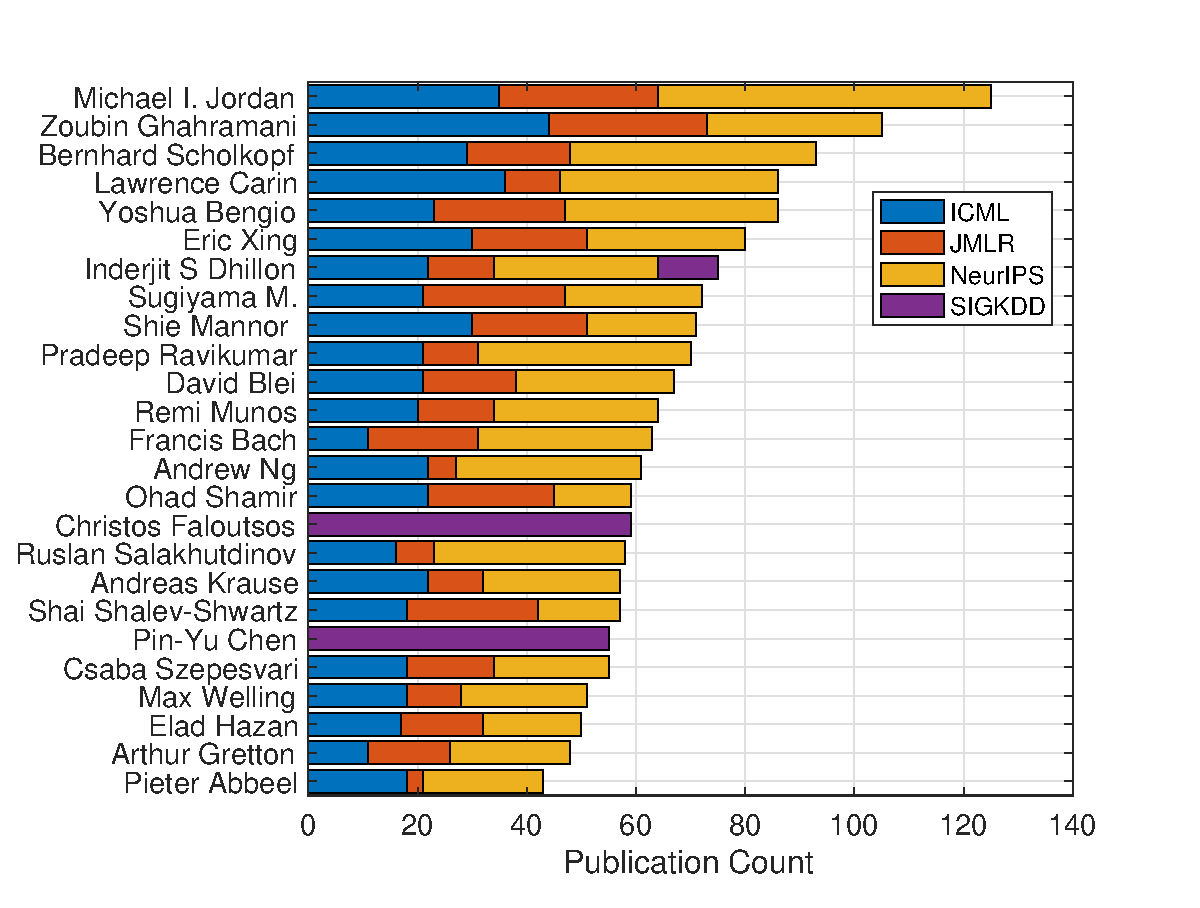
\includegraphics[width=0.45\textwidth]{figure/Total_pub_auth.eps}
	\end{center}
	\caption{Authors with the highest publication count during 2004--2019. \textit{Most of the authors are performing equally well in ICML, JMLR, and NeurIPS but have not published a single paper in SIGKDD.}}
% 	\ignacio{change legend to SIGKDD}}}
	\label{fig:author_total}
\end{figure}

A simple measure would be publication count,  as listed in Figure \ref{fig:author_total}. Most of the authors are performing equally well in ICML, JMLR, and NeurIPS but have not published a single paper in SIGKDD. Only two of the top author have focally published in SIGKDD. Inderjit S. Dhillon is the only author who have performed equally well across all of the understudy venues. Figure \ref{fig:authors_top} also shows the top authors individually in all of the four venues.
% \gareth{Could we add another fig next to Fig 2? This would be a 4xCDFs showing the distribution of papers-per-author across the entire dataset. This would provide context for this top 25 list (i.e. I'm guessing most authors only have 1 paper)}

\begin{figure*}[!htpb]
	\begin{center}
			\subfloat[]{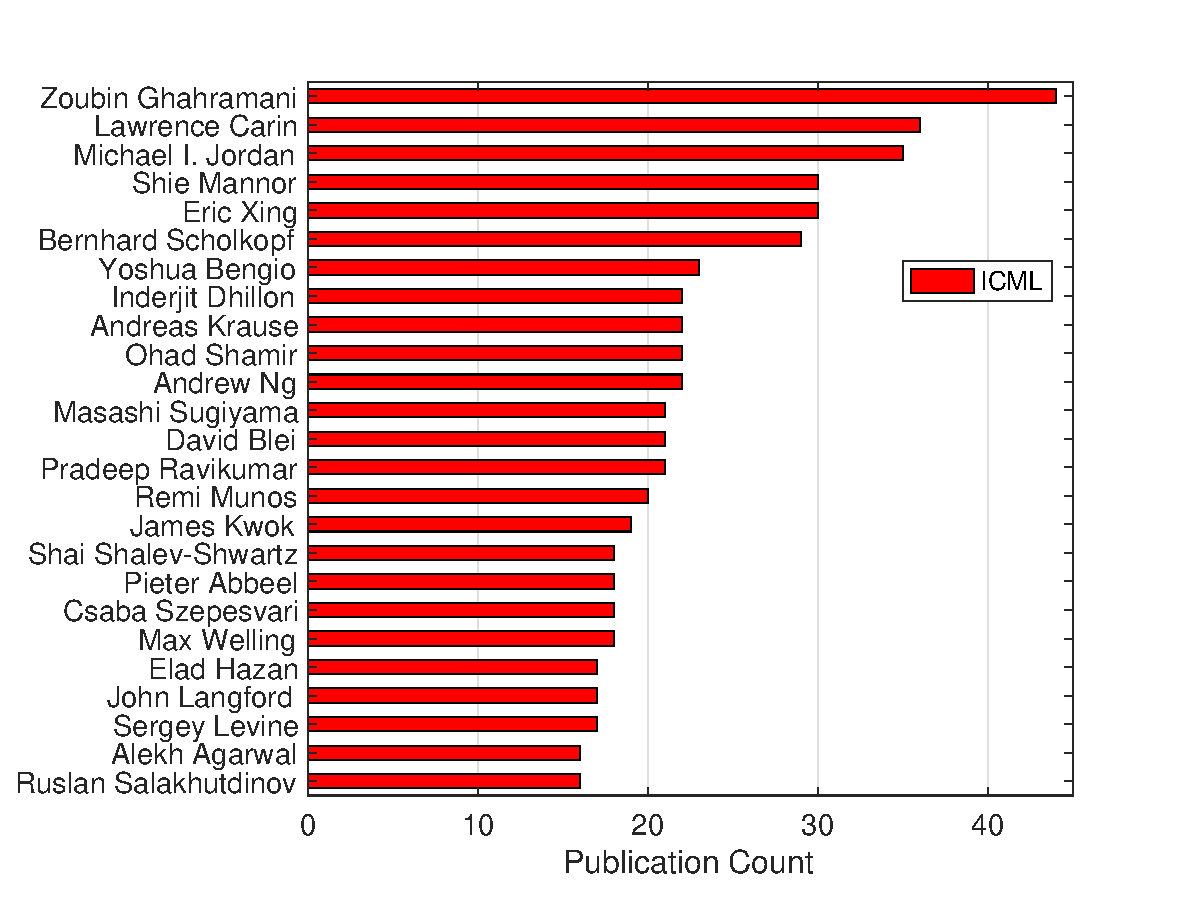
\includegraphics[width=0.45\textwidth]{figure/Freq_ICML.eps}}
	\subfloat[]{\includegraphics[width=0.45\textwidth]{figure/authors_freq_JMLR.eps}}\\
		\subfloat[]{\includegraphics[width=0.45\textwidth]{figure/author_freq_NIPS.eps}}
	\subfloat[]{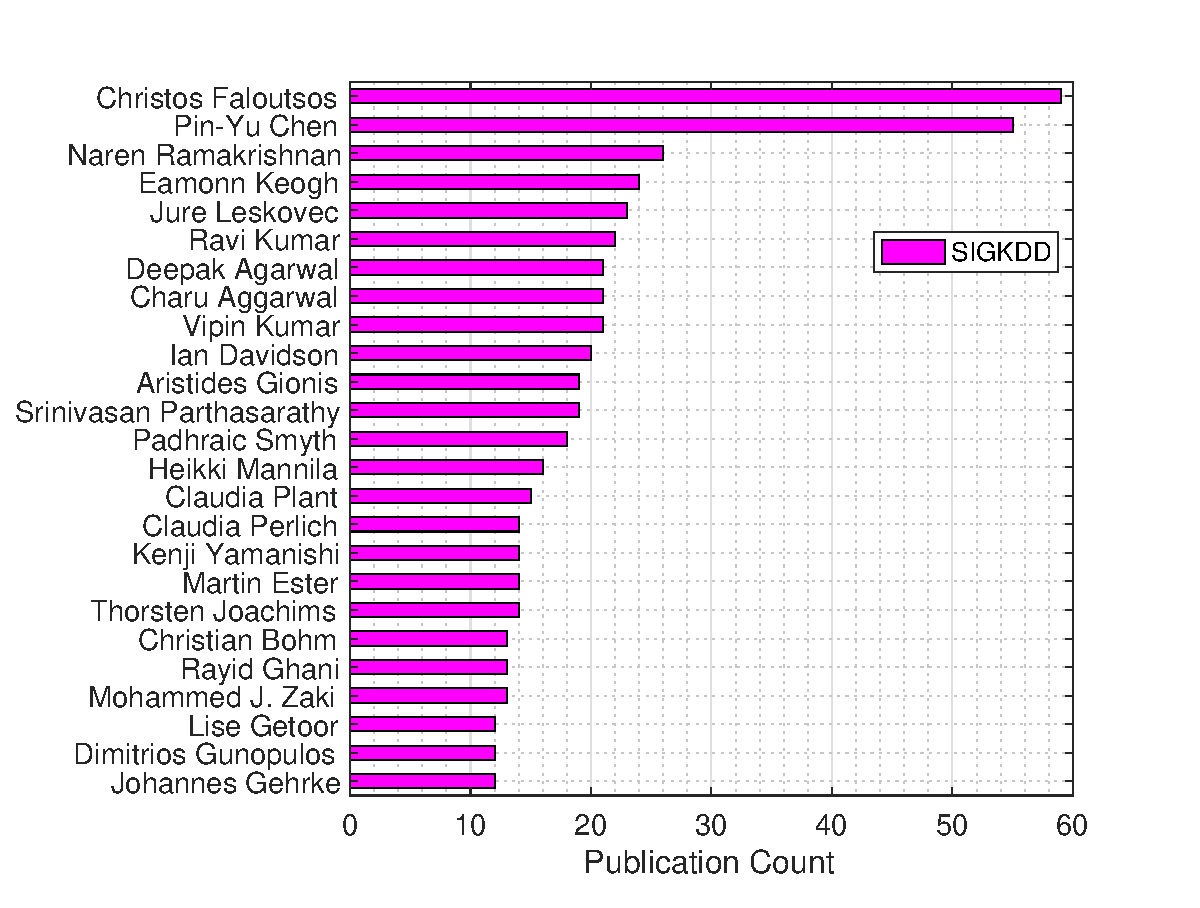
\includegraphics[width=0.45\textwidth]{figure/Author_freq_SIGKDD.eps}}
	\end{center}
	\caption{Most-published authors during 2004--2019, according to article count. \textit{Interestingly, there are major overlap in theoretical study based articles, supporting a ``Renaissance Man'' hypothesis implying that there are many authors who are equally extremely prolific across the theoretical studies based venues.}}
	\label{fig:authors_top}
\end{figure*}

\begin{figure*}[!htbp]
	\begin{center}
		\subfloat[]{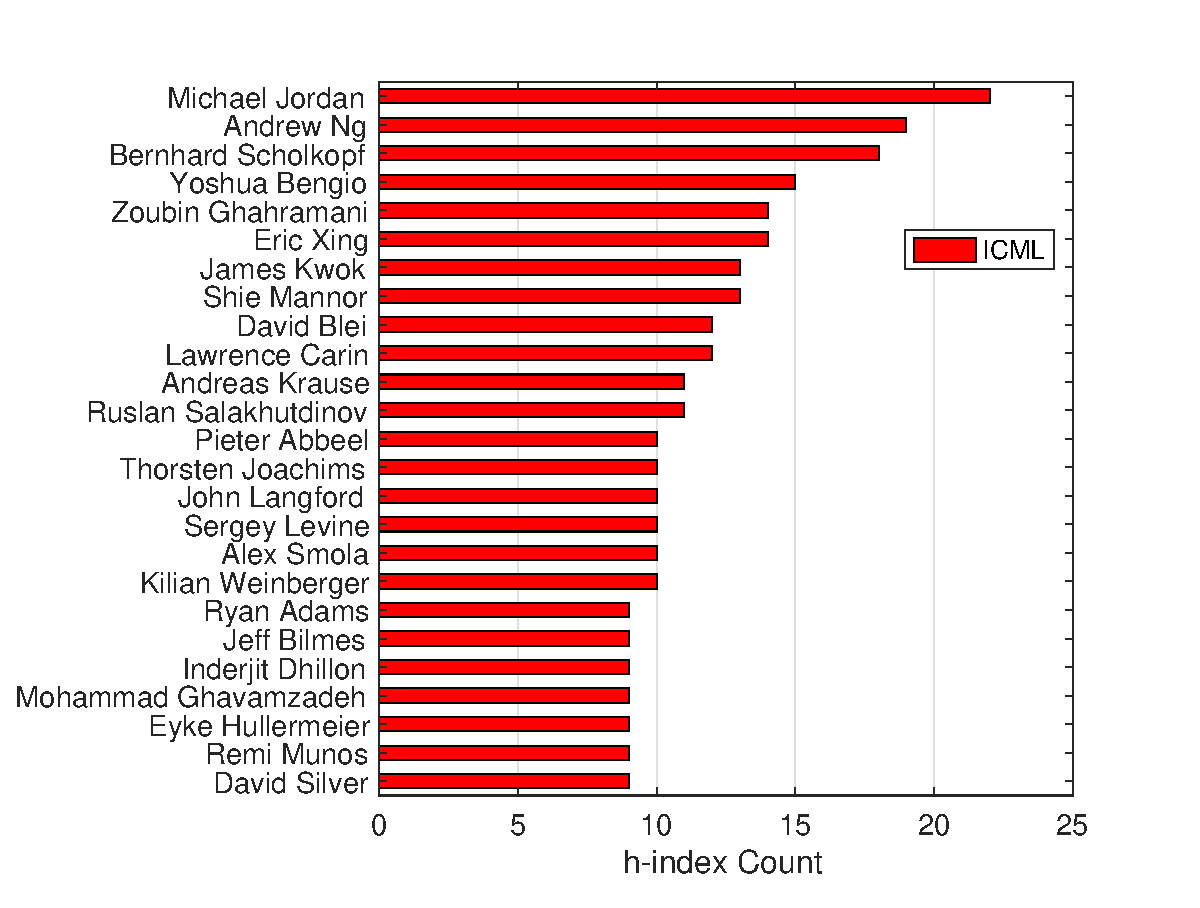
\includegraphics[width=0.45\textwidth]{figure/h-index_ICML.eps}}
	\subfloat[]{\includegraphics[width=0.45\textwidth]{figure/authors_freq_hindex_JMLR.eps}}\\
		\subfloat[]{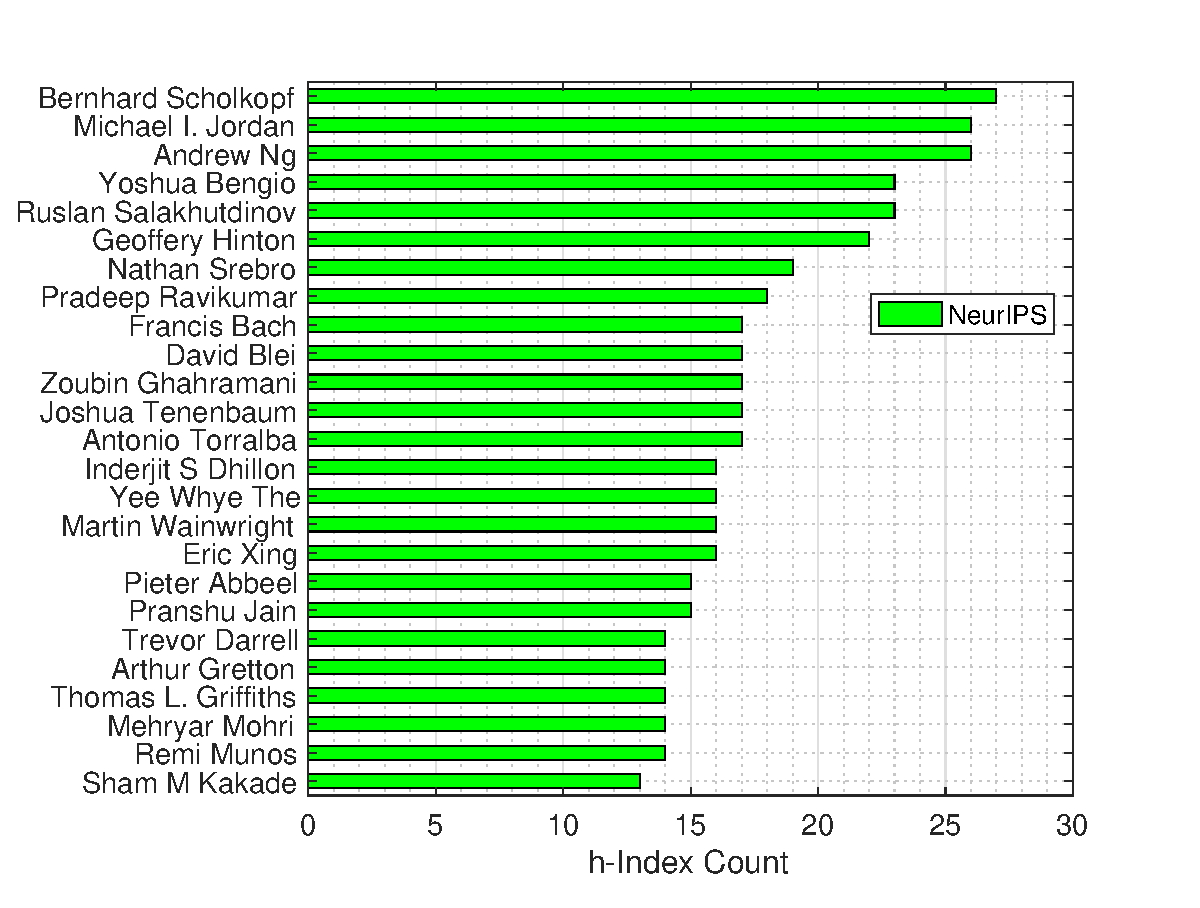
\includegraphics[width=0.45\textwidth]{figure/auth_h-index_NIPS.eps}}
	\subfloat[]{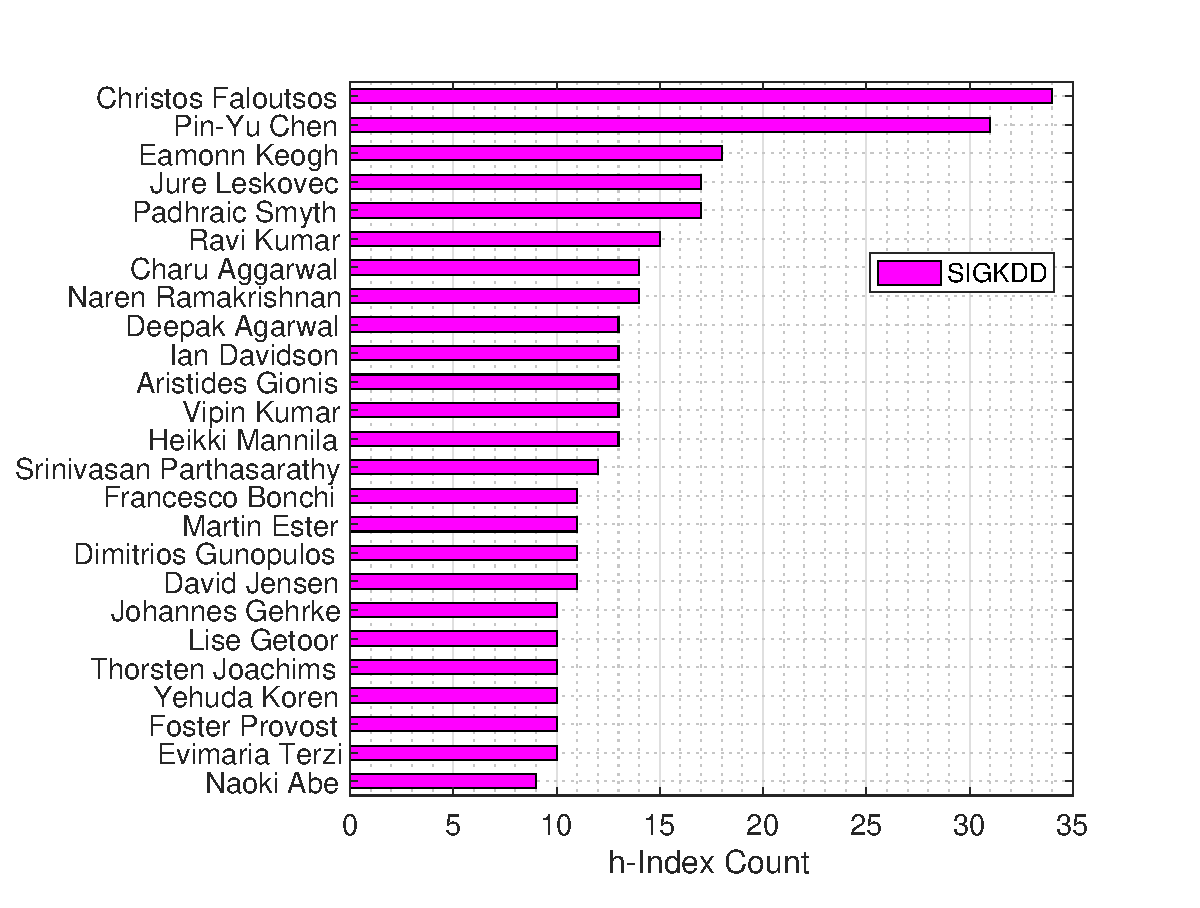
\includegraphics[width=0.45\textwidth]{figure/Author_hindex_SIGKDD.eps}}
	\end{center}
	\caption{Authors with the highest h-index during 2004--2019. \textit{The most-published list and authors with the highest h-index are almost identical in both machine learning and neural networks based studies (i.e. ICML, JMLR, and NeurIPS) indicating a strong relationship between numbers of articles published and h-index. Similar trend is also observed in SIGKDD as well.}}
	\label{fig:cited_top_hindex}
\end{figure*}


The h-index is also another widely used metric where \textit{h} tells us that \textit{h} articles of a researcher have \textit{h} citations \citep{hirsch2005index}. Using the h-index of only ICML, JMLR, NeurIPS, and SIGKDD, we can observe which authors are publishing highly cited research in these venues. 
Figure \ref{fig:cited_top_hindex} shows the authors in our dataset with the highest h-index, and how the top highest publication counts are from the authors with the highest h-index across all discussed genre of articles. The data confirms that the top authors (measured by publication count) are the ones who have significant research contributions in terms of publication count as well as citation count.



\subsubsection{Country Based Productivity Analysis}

In a research domain, some countries play a pivotal role in driving the ongoing advancements in that field. Figure \ref{fig:country_top} shows the rank of different countries based on published articles in all of the four datasets using a global heat map. 


Data shows that the United States and United Kingdom are in the first two highest position in all four venues in terms of publication count. Other top countries include Canada, China, France, and the Germany in all of the four venues. This trend shows that only a handful of countries are contributing disproportionately in development of machine learning research. There is an absence of scholarship from Africa in all of these venues where as Afro-ethnic researcher are contributing quality research with affiliation of other countries in all of the four venues. Similarly, NeurIPS is not geographically diverse as other countries.


The differences in a country's publications in the various venues can partly be attributed to different publication cultures arising from different incentives for faculty promotion/assessment. Some countries in North America and parts of Europe (e.g., USA and UK) give more weight to top-tier conferences (like ICML, NeurIPS etc.) in their assessment criteria while many others in parts of Asia and southern Europe (e.g., India, Malaysia, France, Spain, Italy) emphasize journal publications. In many cases, extended versions of conference papers in the machine learning domain are published in journals such as JMLR.

\begin{figure*}[!htbp]
	\centering
	\subfloat[]{\includegraphics[width=0.45\textwidth]{figure/ICML_full_final.png}}
	\subfloat[]{\includegraphics[width=0.45\textwidth]{figure/JMLR_Full_final.png}}\\
		\subfloat[]{\includegraphics[width=0.45\textwidth]{figure/NeuIPS_Full_final.png}}
	\subfloat[]{\includegraphics[width=0.45\textwidth]{figure/SIGKDD_full_final.png}}
	\caption{Rank of different countries based on publication count in all of four venues. \textit{Although most countries have similar productivity in these venues, there are notable exceptions where the publication trends are quite dissimilar.}}
	\label{fig:country_top}
\end{figure*}

From the above analysis, it is evident that all of the four venues attract attention from significant researchers in the field. Hence, we posit that it may be difficult for new emerging scholars to publish in such venues. 
Indeed, anecdotally, this is often claimed.
To identify emerging authors, we extract all papers with: $(i)$ authors who have never published in the venue before; and $(ii)$ authors who do not have any co-authors who have already published in the venue. 
Figure \ref{fig:country_emer} shows the distribution of emerging authors in all venues conferences during 2004--2019.


\begin{figure*}[!htbp]
	\centering
	\subfloat[]{\includegraphics[width=0.45\textwidth]{figure/ICML_emer_final.png}}
	\subfloat[]{\includegraphics[width=0.45\textwidth]{figure/JMLR_emer_final.png}}\\
		\subfloat[]{\includegraphics[width=0.45\textwidth]{figure/NeurIPS_emer_final.png}}
	\subfloat[]{\includegraphics[width=0.45\textwidth]{figure/SIGKDD_emer_final.png}}
	\caption{Rank of different countries based on publication count from first-time contributor in all of four venues. \textit{ Those include $(i)$ authors who have never published in the venue before; and $(ii)$ authors who do not have any co-authors who have already published in the venue.}}
	\label{fig:country_emer}
\end{figure*}

\begin{figure*}[!htbp]
	\centering
	\subfloat[]{\includegraphics[width=0.45\textwidth]{figure/COUNTRY_GRAPH_ICML_u.png}}
	\subfloat[]{\includegraphics[width=0.45\textwidth]{figure/country_al.png}}\\
		\subfloat[]{\includegraphics[width=0.45\textwidth]{figure/countries_NIPS.png}}
	\subfloat[]{\includegraphics[width=0.45\textwidth]{figure/Country_SIGKDD.png}}
	\caption{Co-authorship network among top countries in (a) ICML; (b) JMLR; (c) NeurIPS; and (d) SIGKDD. Node size indicates the number of links with other nodes in the co-authorship network and the node color represents cluster membership.}
	\label{fig:country_top_gephi}
\end{figure*}


We next inspect the collaborations that took place between these countries. Figure \ref{fig:country_top_gephi} shows the co-authorship network of top countries in all four venues. 

In ICML, JMLR, and NeurIPS, the top five countries have significant co-authorship activities among themselves, thus they are clustered in a single group. In SIGKDD, top publishing are clustered in two clusters. With the advancement of information and communication technologies, researchers from various countries now have new ways to work with each other. Top countries enjoy the share of publication from their authors, and in addition a contribution from authors from collaborating countries. 




\subsubsection{Institutional and Author Based Collaborations}
This subsection presents the varying trends of collaborations among the institutes and authors in ICML, JMLR, NeurIPS, and SIGKDD over the period from 2004 to 2019. We will address several important questions relating to the collaboration patterns of institutes and countries; the most influential institutes and authors in all of the four venues; and whether influential institutes and authors tend to work as collaborators. To observe collaborative relations among the top researchers in all of four venues, we generate undirected graphs of co-authors and identify clusters using modularity class partitioning. We used undirected graphs to remove duplicate links among publishing entities. 

Figure \ref{fig:authors_top_gephi} presents the clusters present in the network. We find 187 different clusters of authors in ICML, 31 clusters in JMLR, 145 clusters in NeurIPS, and 83 clusters in SIGKDD. To improve the visualization, we only include authors who have more than five articles in ICML, JMLR, NeurIPS, and SIGKDD. 


\begin{figure*}[!htbp]
	\centering
	\subfloat[]{\includegraphics[width=0.45\textwidth]{figure/authors_graph_ICML_u.png}}
	\subfloat[]{\includegraphics[width=0.45\textwidth]{figure/authors_graph_JMLR_u.png}}\\
		\subfloat[]{\includegraphics[width=0.45\textwidth]{figure/auth_AL_NIPS_u.png}}
	\subfloat[]{\includegraphics[width=0.45\textwidth]{figure/authors_al_SIGKDD.png}}
	\caption{Co-authorship network among top authors in the field of machine learning (a) ICML; (b) JMLR; (c) NeurIPS; and (d) SIGKDD. Only those who have authored at least 5 articles are kept in clusters.}
	\label{fig:authors_top_gephi}
\end{figure*}


Published research is a crucial factor in determining the quality of education and research at any institute. Figure \ref{fig:inst_top} shows a similar result for the top institutes. We performed a clustering analysis using modularity class algorithm over ICML, JMLR, NeurIPS, and SIGKDD articles. 

Figure \ref{fig:inst_top_gephi} shows a similar result for all of the four venues datasets. In all venues, the top publishing institutes are clustered into three groups according to their publishing behavior. In all of the four venues, CMU, UC Berkeley, Stanford University, and MIT, both in the United States, showed a significant co-authorship pattern. 



\begin{figure*}[!htbp]
	\begin{center}
		\subfloat[]{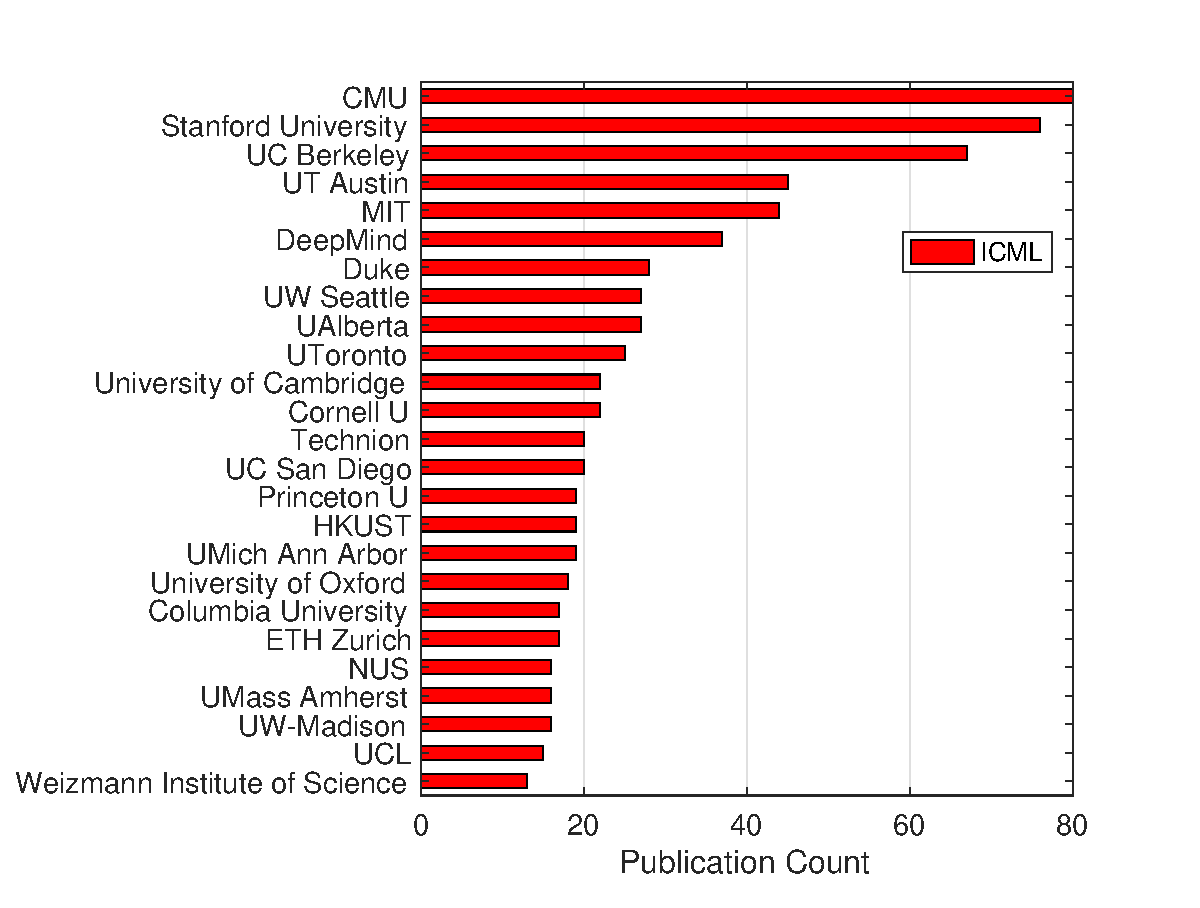
\includegraphics[width=0.45\textwidth]{figure/Insti_Freq_ICML.eps}}
	\subfloat[]{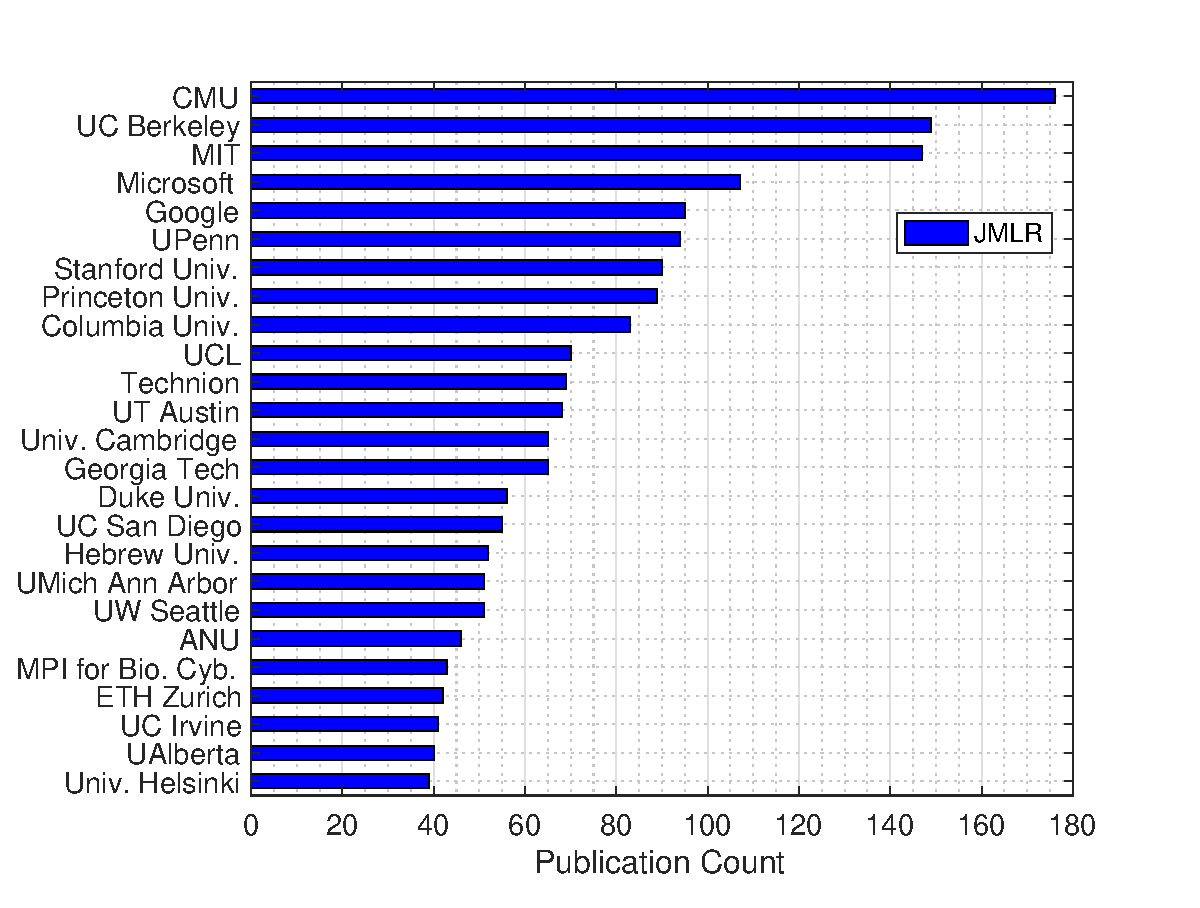
\includegraphics[width=0.45\textwidth]{figure/institutes_freq_JMLR.eps}}\\
		\subfloat[]{\includegraphics[width=0.45\textwidth]{figure/institutes_NIPS.eps}}
	\subfloat[]{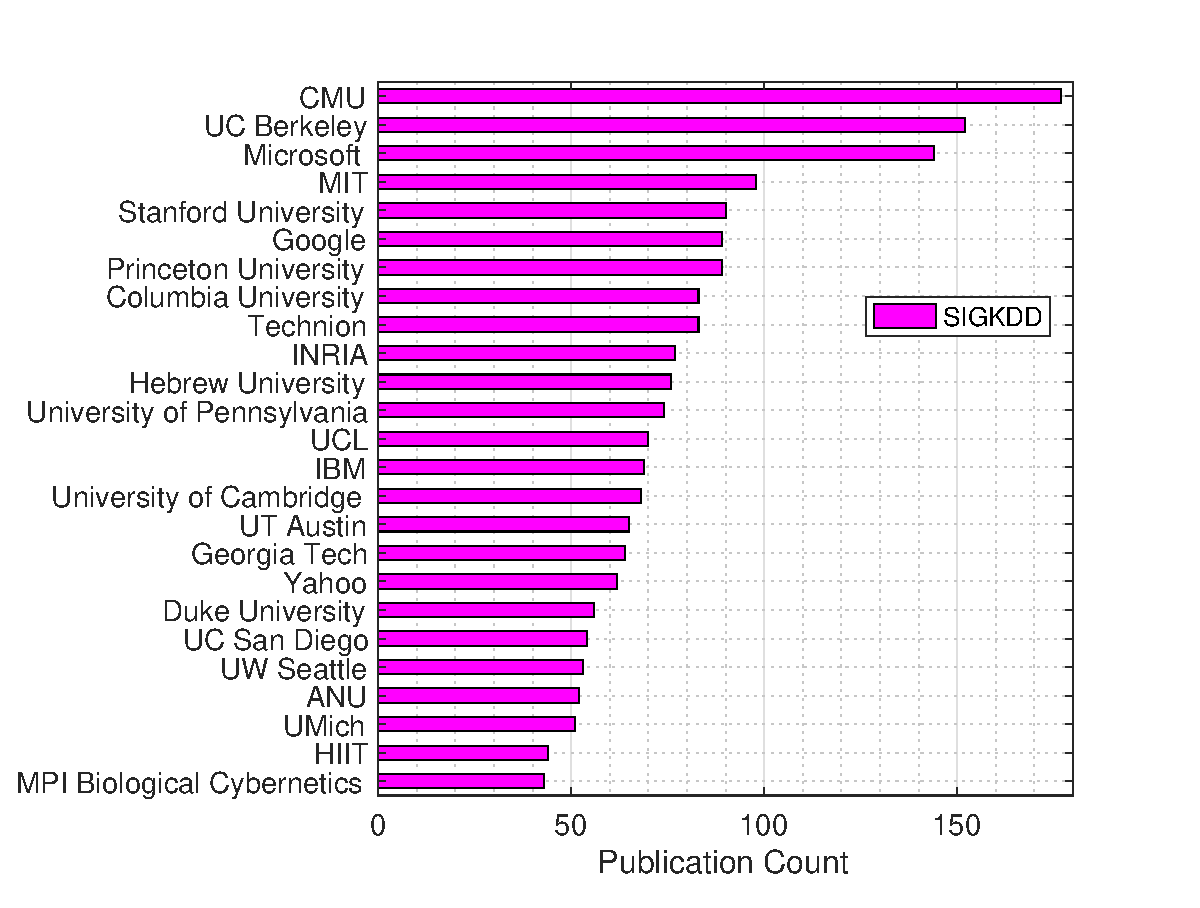
\includegraphics[width=0.45\textwidth]{figure/Institutes_freq_SIGKDD.eps}}
	\end{center}
	\caption{Most-published institutes during 2004--2019, according to their article count. \textit{In all of the four venues, academic institutes are publishing more significant contributors as compared industrial contributors. CMU tops all four venues followed by Stanford in two venues and by UC Berkeley in the other two venues.}}
	\label{fig:inst_top}
\end{figure*}


\begin{figure*}[!htbp]
	\centering
	\subfloat[]{\includegraphics[width=0.45\textwidth]{figure/insti_graph_ICML.png}}
	\subfloat[]{\includegraphics[width=0.45\textwidth]{figure/institute_al_JMLR_u_al.png}}\\
		\subfloat[]{\includegraphics[width=0.45\textwidth]{figure/institutes_NIPS_u_al.png}}
	\subfloat[]{\includegraphics[width=0.45\textwidth]{figure/Institutes_SIGKDD_u_al.png}}
	\caption{Co-authorship network among top institutes in (a) ICML; (b) JMLR; (c) NeurIPS; and (d) SIGKDD (with 10 minimum published articles). \textit{Distinct patterns can be observed in all four venues: academic institutes are prominent in all across the dataset.}}
	\label{fig:inst_top_gephi}
\end{figure*}

To remove the weak links, in all venues we set the degree threshold to 10. We found 21 different clusters of institutes in ICML, 84 clusters in JMLR, 42 clusters in NeurIPS, and 29 clusters in SIGKDD. To improve the visualization, we only include institutes who have more than 10 articles in all four venues. Social network analysis has shown us the hidden relations between the top authors of ICML, JMLR, NeurIPS, and SIGKDD, and we conclude that most of the top authors (measured by their publication count in all four venues) are clustered together because either they have strong collaboration behavior with each other or common co-author in-between.

\subsection{Referencing Patterns}
First, we extract the references from all papers and create a citation graph, as we are curious to understand how all ICML, JMLR, NeurIPS, and SIGKDD cite each other.
Figure \ref{fig:top_flow_venues_c} is a Sankey diagram, showing the fraction of papers that reference papers from all of the four venues (left), as well as the other papers that in turn cite the papers in our dataset (right). 

Note that this covers all of the four venues. 
Interesting patterns emerge from this analysis. 
Most noteworthy is the bias for citing papers from the same venue. For example, 26\% of references in ICML papers are for other papers previously published in ICML. Similar trend are observed for other venues as well. 


In contrast, a far more diverse body of publication outlets list papers from our dataset in their references. This is particularly for other conferences (57\% of the papers in our dataset which cite our selected venues are actually conferences, rather than journals). 
Major citers of our dataset papers include Neurocomputing, ICLR, CVPR, and IEEE Access.
This trend is perhaps intuitive as all of the four venues are considered among the most prestigious outlets, and therefore it is unsurprising that a wide diversity of venues cite such papers. 
All that said, it is clear that a number of other publication venues feature heavily in the bibliographies of our dataset's papers, and these are dominated by conferences rather than journals.


\begin{figure}[H]
	\centering
	\includegraphics[width=0.45\textwidth]{figure/sanky_all.png}
	\caption{The distribution of references and citations in ICML, JMLR, NeurIPS, and SIGKDD. The left input shows the conferences that are referenced by all of the four venue papers; the right output shows which papers cite papers from our dataset. \emph{Major source of references and citations in our dataset are from conferences.} }
	\label{fig:top_flow_venues_c}
\end{figure}




\section{Content Based Analysis and Findings}
\label{sec:content}

This section keyword-based analysis, based on index keywords; We address questions such as, what topics are discussed by top authors in all of the four venues?

\subsection{Keyword-based analysis of articles} 



Investigating the popular topics is considered to be one of the best ways of studying the paradigm shifts in any research field. 
\begin{figure*}[!htbp]
	\begin{center}
		\subfloat[]{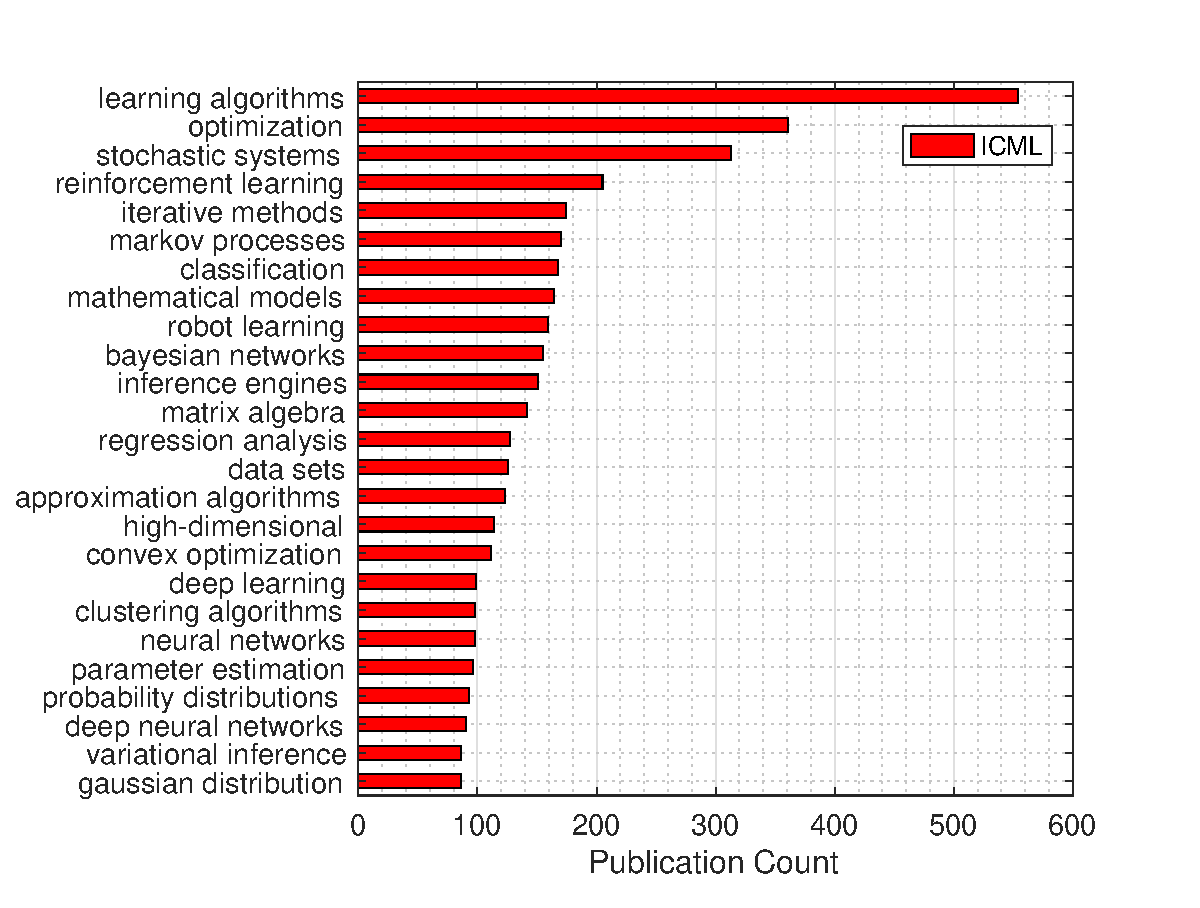
\includegraphics[width=0.45\textwidth]{figure/ICML_Keyword_Freq.eps}}
	\subfloat[]{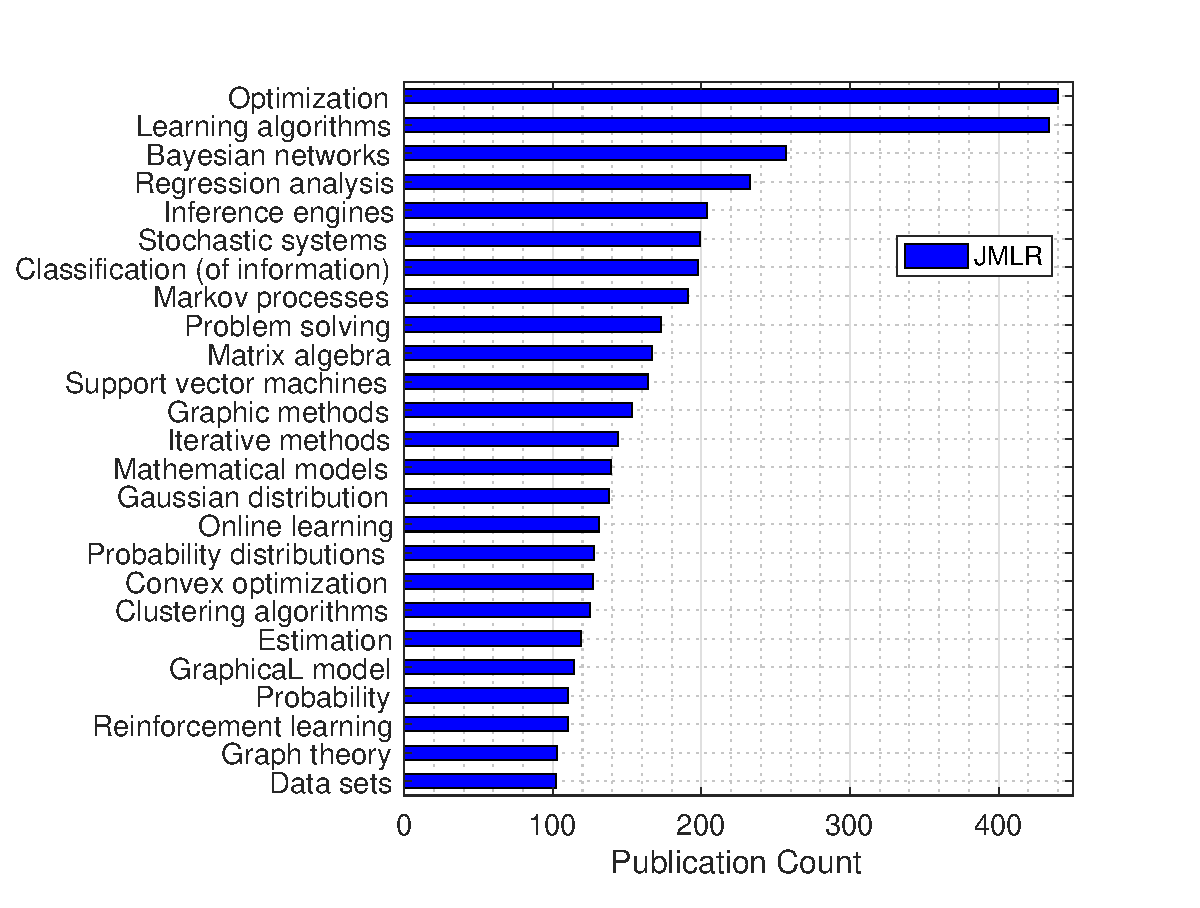
\includegraphics[width=0.45\textwidth]{figure/keywords_freq_JMLR.eps}}\\
		\subfloat[]{\includegraphics[width=0.45\textwidth]{figure/keyword_freq_NIPS.eps}}
	\subfloat[]{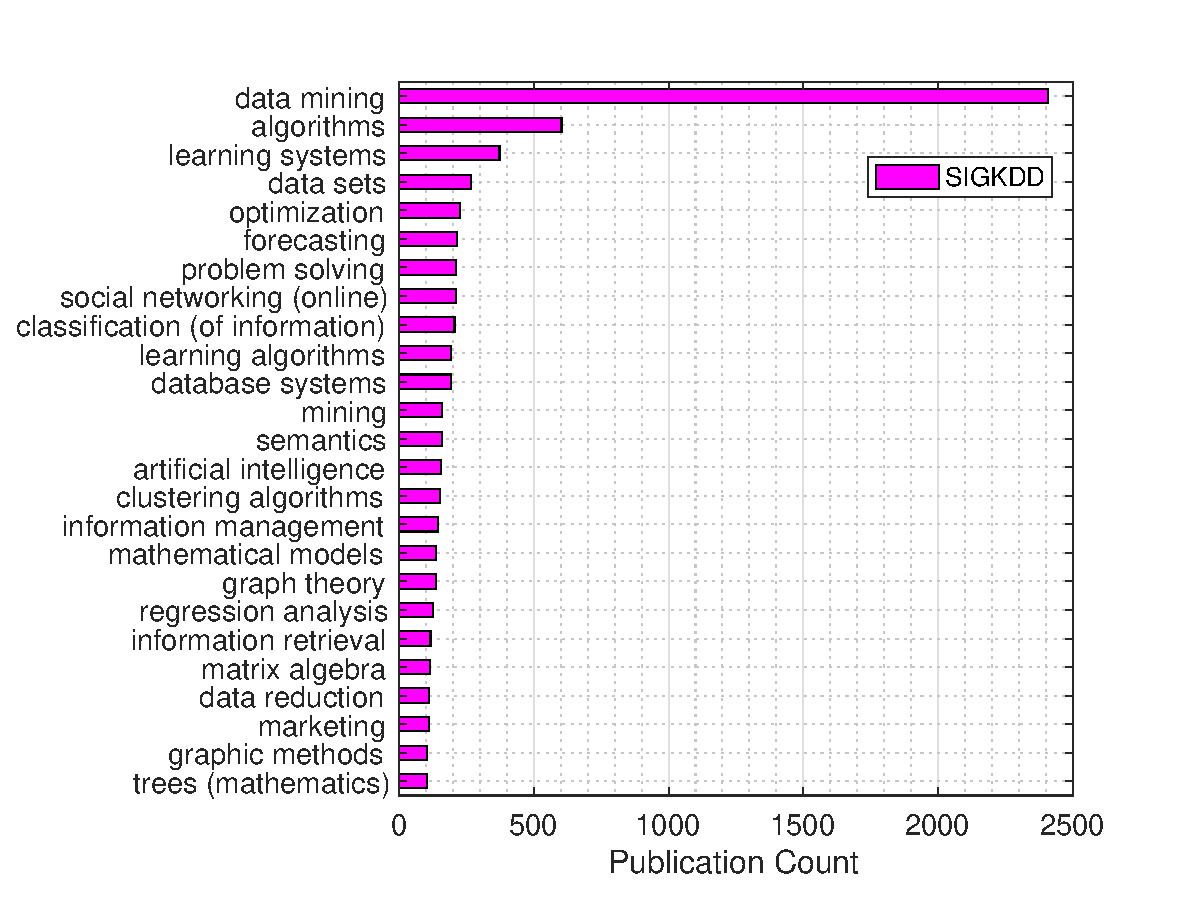
\includegraphics[width=0.45\textwidth]{figure/Keyword_freq_SIGKDD.eps}}
	\end{center}
	\caption{Most popular topics in ICML, JMLR, NeurIPS, and SIGKDD and their article count during 2004--2019, in terms of article count (cf. Figure \ref{fig:cited_top_keywords}, in which keywords of the most-cited articles are listed.)}
	\label{fig:keywords_top}
\end{figure*}

It is helpful in describing the research trends of a field. In this sub-section, we use ICML, JMLR, NeurIPS, and SIGKDD data to analyze the popular topics in the field of machine learning. We have described the top popular topics discussed in these articles in machine learning. This approach provides a holistic overview of research trends in machine learning since it covers both theoretical and application based articles.

Figure \ref{fig:keywords_top} represents the most popular topics in machine learning, according to the our dataset. ``Learning Systems'', ``Learning Algorithms'', ``Optimization'', and ``Data mining''. 


\subsection{Keyword co-occurrence analysis}
Keyword co-occurrence analysis helps researchers to find a publication venue's most common topics. 
\begin{figure*}[!htbp]
	\centering
	\subfloat[]{\includegraphics[width=0.45\textwidth]{figure/keyword_wo_large_ICML_u.png}}
	\subfloat[]{\includegraphics[width=0.45\textwidth]{figure/keyword_al_JMLR_u.png}}\\
		\subfloat[]{\includegraphics[width=0.45\textwidth]{figure/keyword_al_NIPS_u.png}}
	\subfloat[]{\includegraphics[width=0.45\textwidth]{figure/keyword_al_SIGKDD_u.png}}
	\caption{Keyword co-occurrence network in which the node size indicates the number of links with other nodes and node color represents cluster membership. \textit{It can be noted that keywords, discussed in our dataset, are typically biased towards algorithms and optimization (solutions and techniques)}.}
	\label{fig:keyword_top_gephi}
\end{figure*}

These analyses also help researchers to find topics and domains that are strongly related to each other. Figure \ref{fig:keyword_top_gephi} is the term co-occurrence map for ICML, JMLR, NeurIPS, and SIGKDD.

There is major overlap in the keywords used in the top-cited articles in all of the four venues. Keywords, discussed in our dataset, are typically biased towards algorithms and optimization (solutions and techniques).

Terms in a larger font size have a higher co-occurrence than other keywords in the graphs. In our dataset, frequently co-occurring terms are "Learning algorithms", "Optimization", "data mining", and "stochastic systems". Top keywords (measured on publication count) in our dataset are clustered in the same groups and have stronger links with each other than with unpopular keywords. This trend shows that in all of the four venues, there are only some top keywords (measured on publication count) which are discussed in most of the articles.



\section{Citation Based Analysis and Findings}
\label{sec:citation}

Citations are used to investigate the contributions of an author, organization, country or publication venue. Citation analysis is an effective tool to rank the productivity of various research bodies. In this section, we address some important bibliometric questions using citation data from ICML, JMLR, NeurIPS, and SIGKDD articles, such as who are the most-cited authors in all of the four venues; whether they have the same h-index as the most-published authors; whether increasing the number of authors affects the number of citations of an article; the most-cited keywords in all of the four venues.


\subsection{Citation Based Analysis of Different Research Entities}
In machine learning, some authors play more significant roles in advancements of the field than others. It is worth observing the impact and usability of their research. 
\begin{figure*}[!htbp]
	\begin{center}
	\subfloat[]{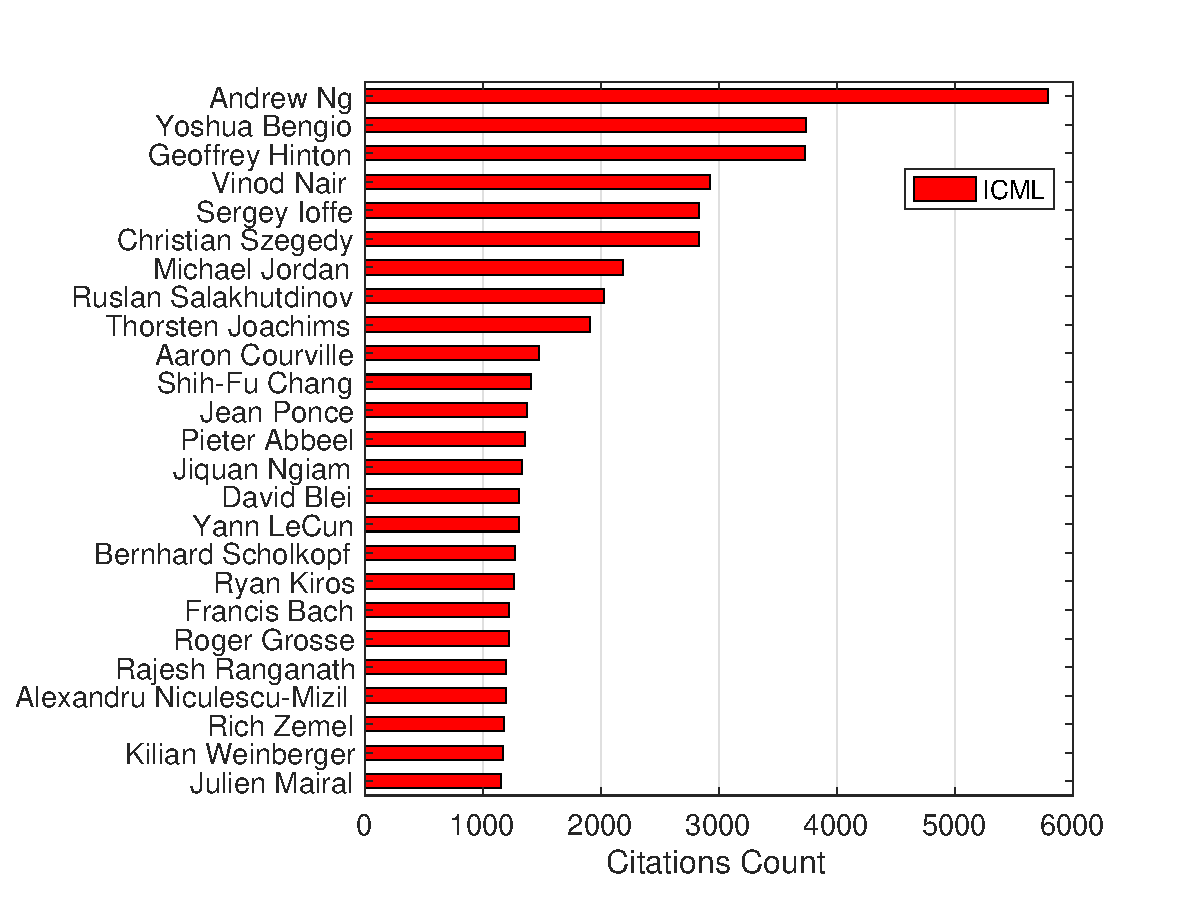
\includegraphics[width=0.45\textwidth]{figure/cite_ICML.eps}}
	\subfloat[]{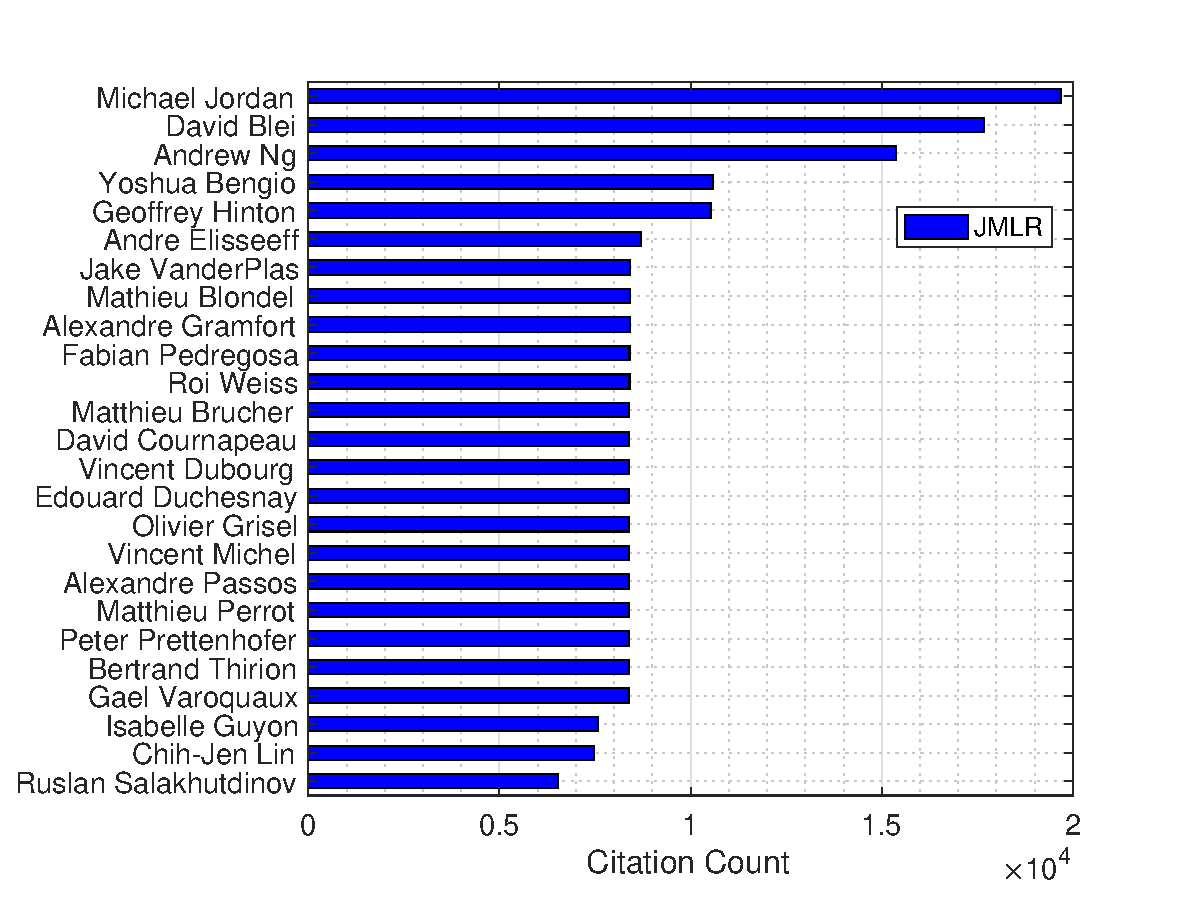
\includegraphics[width=0.45\textwidth]{figure/authors_freq_cite_JMLR.eps}}\\
		\subfloat[]{\includegraphics[width=0.45\textwidth]{figure/authors_cite_NIPS.eps}}
	\subfloat[]{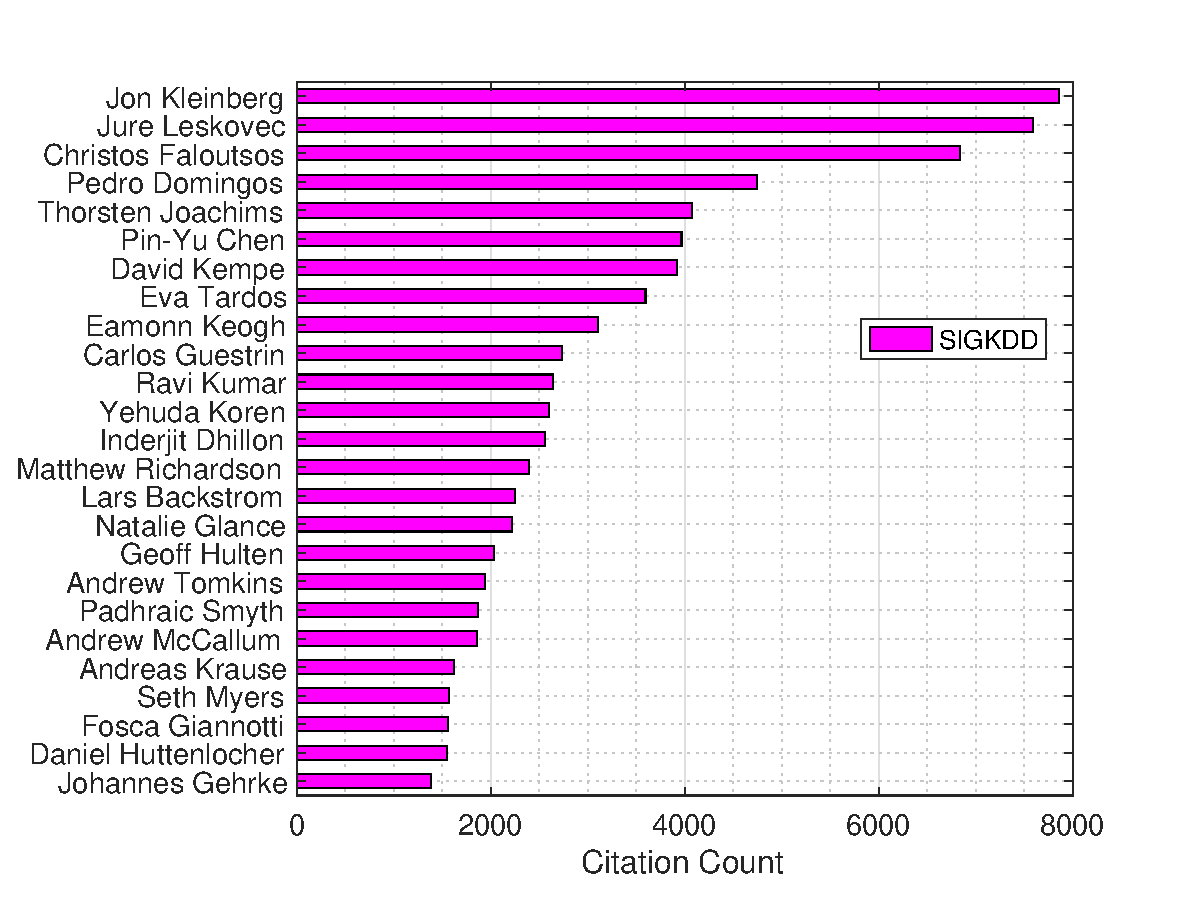
\includegraphics[width=0.45\textwidth]{figure/Author_cite_SIGKDD.eps}}
	\end{center}
	\caption{Most-cited authors. \textit{We see that the most-cited NeurIPS articles tend to have more citations as compared to other three venues.}}
	\label{fig:cited_top}
\end{figure*}


Figure \ref{fig:cited_top} shows the most-cited authors in all four venues from 2004 to 2019. From Figure \ref{fig:cited_top} and Figure \ref{fig:authors_top}, it can be observed that the top most-published authors and the top most-cited authors in all four venues are significantly different. 

Citations do not entirely represent the significance of the research undertaken by a researcher. There are many parameters to analyze its significance, but the h-index is the most widely used, and it is a better measure of an author's significance in a field than a simple citation count. 

Figure \ref{fig:cited_top_hindex} shows the authors in ICML, JMLR, NeurIPS, and SIGKDD with the highest h-index, and how the top highest publication counts are from the top authors with the highest h-index in all four venues. The data confirms that the top authors (measured by publication count) are the ones who have significant research contributions in terms of publication count as well as citation count.

Figure \ref{fig:cited_top_keywords} shows the most cited keywords in our dataset. We can observe that most cited keywords in all of the four venues are significantly different from most published ones.

\begin{figure*}[!htbp]
	\begin{center}
		\subfloat[]{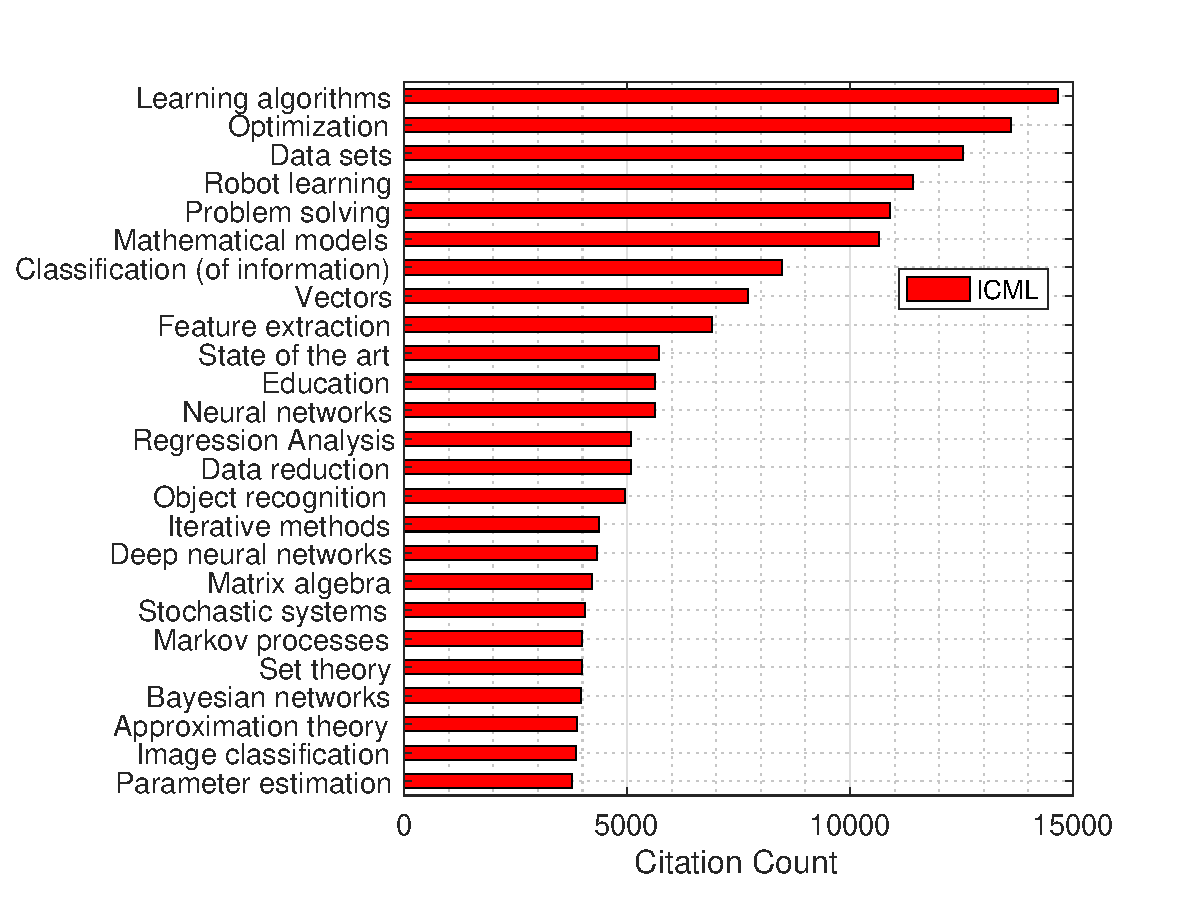
\includegraphics[width=0.45\textwidth]{figure/ICML_keyword_cite.eps}}
	\subfloat[]{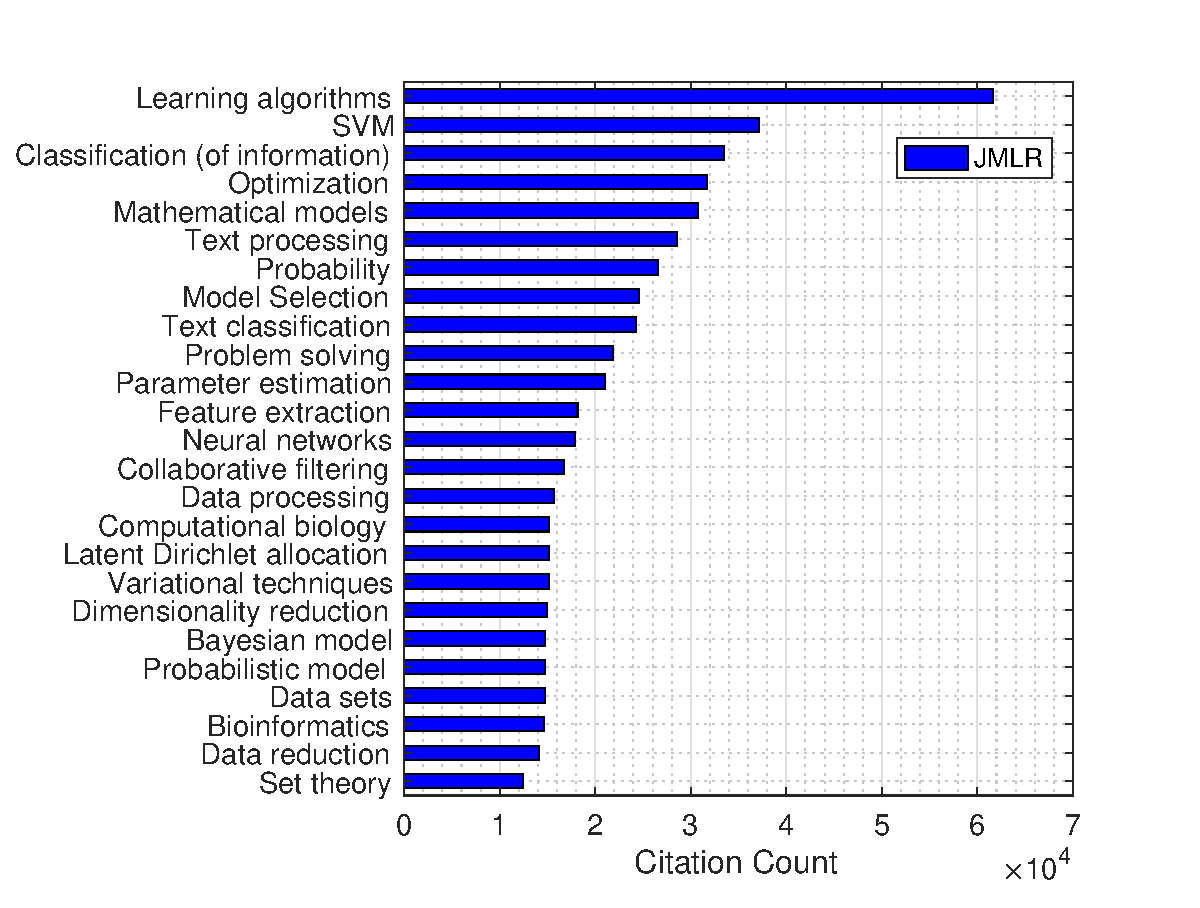
\includegraphics[width=0.45\textwidth]{figure/keywords_cite_JMLR.eps}}\\
		\subfloat[]{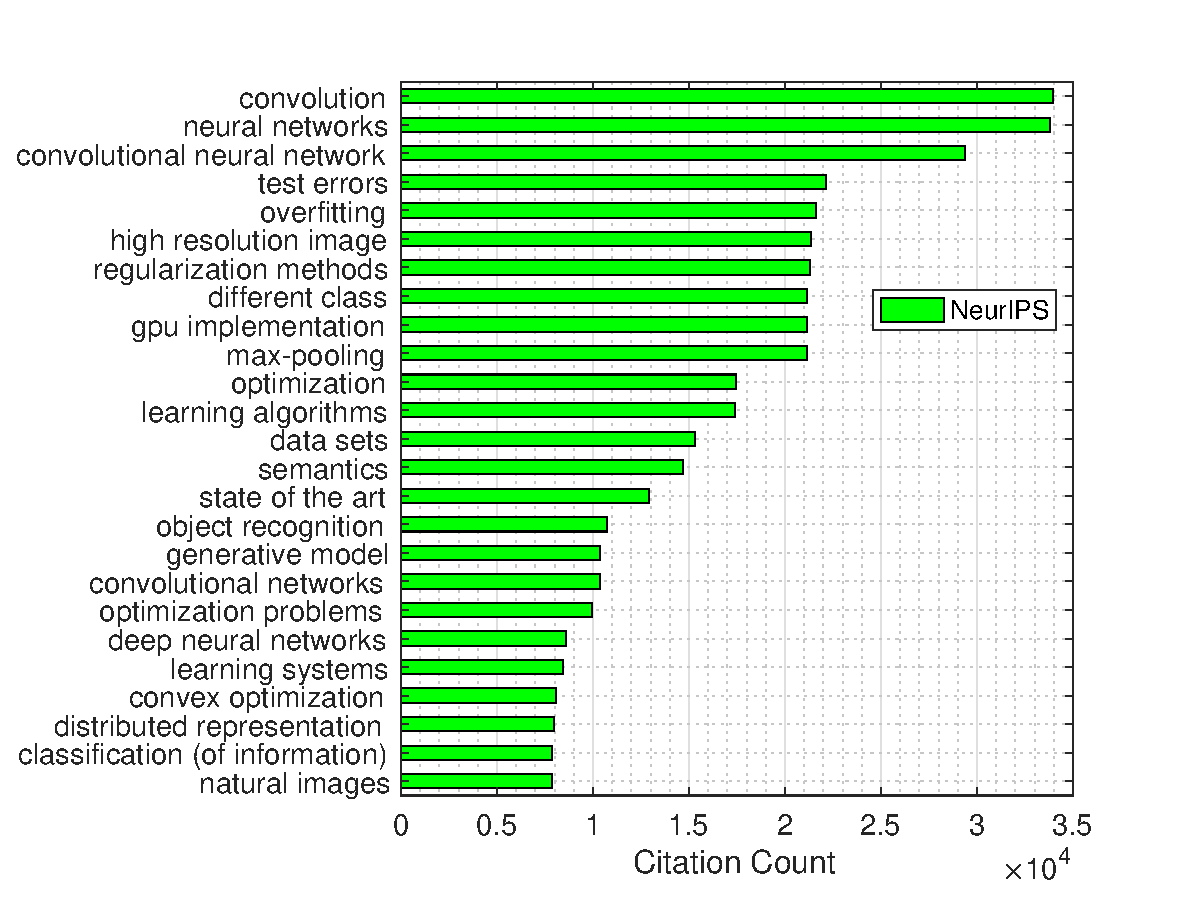
\includegraphics[width=0.45\textwidth]{figure/keyword_cite_NIPS.eps}}
	\subfloat[]{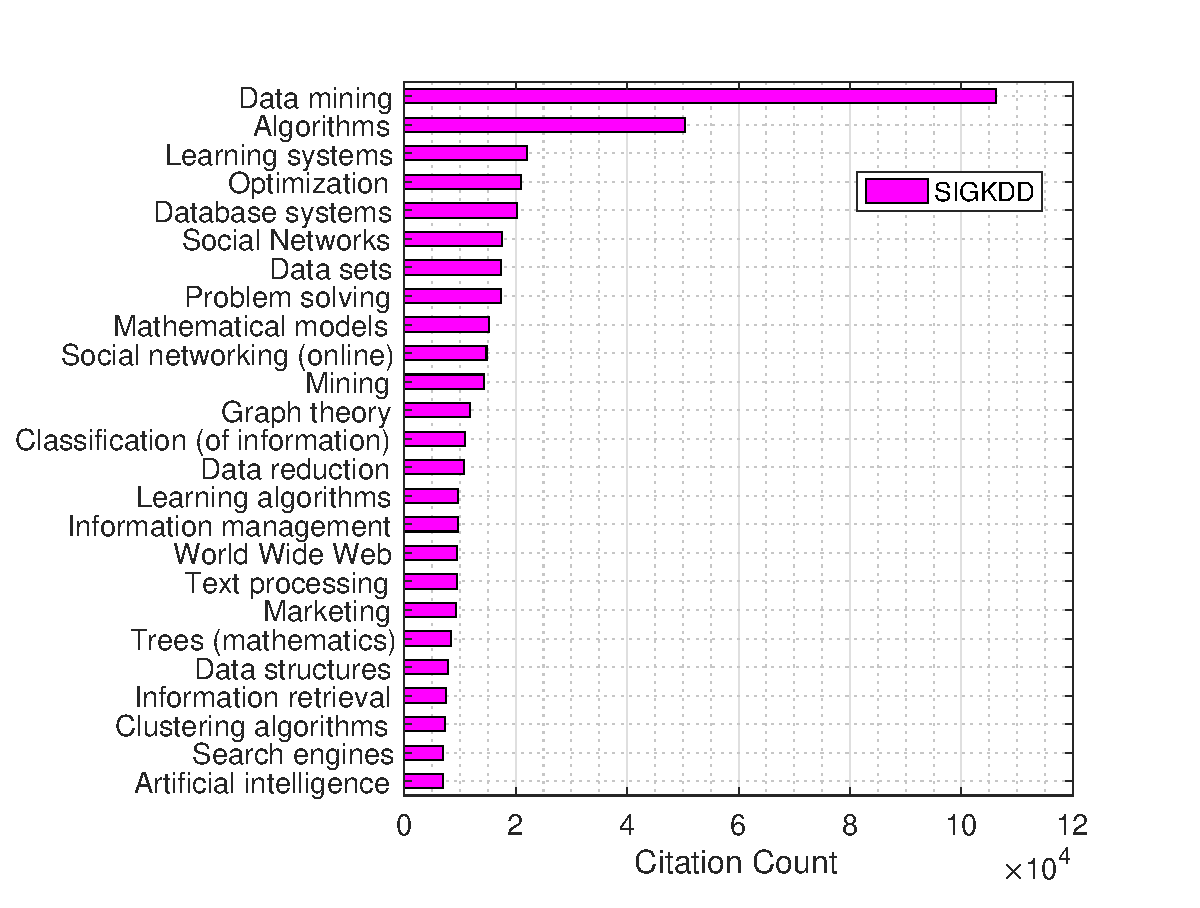
\includegraphics[width=0.45\textwidth]{figure/keyword_cite_SIGKDD.eps}}
	\end{center}
	\caption{Most-cited keywords. \textit{It is noticeable that there is negligible overlap in the keywords used in all discussed venues.}}
	\label{fig:cited_top_keywords}
\end{figure*}

\clearpage
\section{Conclusions}
\label{sec:conclusion}

In this paper, we have performed an in-depth bibliometric study of the publication trends in machine learning literature using article content and metadata of four important machine learning periodicals---International Conference on Machine Learning (ICML), Journal of Machine Learning Research (JMLR), Conference on Neural Information Processing Systems (NeurIPS), and SIGKDD Conference on Knowledge Discovery and Data Mining (KDD)---gathered over the time period 2004--2018.  Our work extends the state of the art in bibliometric analysis of machine learning literature by presented comprehensive analyses that shed light on the publication patterns in these venues including which kinds of articles are published where; how are journal and conference publications different in this area; and which different authors, institutes, and countries have been successful in these venues (and how). We believe that our analyses provide an insightful look into the publication culture in the machine learning community and can help develop a more nuanced understanding of this research field especially in the light of the limited existing bibliometric work that focused on the machine learning community. In this regard, we have also publicly shared our dataset that includes content, metadata, and citation-related information related to the articles published from 2004 to 2018 in ICML, JMLR, NeurIPS, and KDD as our contribution to the research community. \footnote{link to be shared}.

	\balance
	\bibliographystyle{ACM-Reference-Format}
	\bibliography{reference}
	%
	%
%	\newpage
%	\input{other}



\end{document}
